\documentclass[10pt,a4paper]{scrartcl}

\usepackage[english]{babel}
\usepackage{glossaries}\usepackage[xindy]{imakeidx}

%Set to 0 for making without examples
%Set to 1 for making with examples
\gdef\conditionmacro{0}

%\newenvironment{example}{
%\ifnum\conditionmacro=1}
%{\fi}

\input{../Headerfiles/Packages}
\input{../Headerfiles/Titles}
\input{../Headerfiles/Commands}
\input{../Headerfiles/ENVIRONMENTS}
\graphicspath{{Pictures/}}
\parindent 0pt

\title{Informatics}
\author{GianAndrea Müller}

\newtheorem{define}{Definition}

\makenoidxglossaries
\newglossaryentry{Algorithm}{name={Algorithm},description={An algorithm is a set of rules that defines a sequence of operations leading to the solution of a problem.}}
\newglossaryentry{Language}{name={Language},description={A programming language is a set of instructions for a computer that can be used to write programs that implement algorithms.}}
\newglossaryentry{Syntax}{name={Syntax},description={The syntax of a computer language is the set of rules that defines the combinations of symbols that are considered to be a correctly structured program in that language. Is a program grammatically correct?}}
\newglossaryentry{Semantics}{name={Semantics},description={The semantics of a computer language define how the language has to be interpreted. What is the meaning of a certain program?}}
\newglossaryentry{Editor}{name={Editor},description={A program that allows writing code. There exist powerful editors that can check syntactical correctness on the fly.}}
\newglossaryentry{Compiler}{name={Compiler},description={A compiler translates a program written in a programming language to machine code, such that it can be executed by the machine.}}
\newglossaryentry{Computer}{name={Computer},description={A computer is a device that is capable of executing machine code.}}
\newglossaryentry{Comments}{name={Comments},description={Comments document the implemented algorithm within the program for the reader. They are ignored by the compiler.}}
\newglossaryentry{IncDir}{name={Include Directives},description={Include directives specify the additional libraries used in a program.}}
\newglossaryentry{Main}{name={The main function},description={The main function exists in every c++-program. It is unique and contains the all instructions necessary to execute the program.}}
\newglossaryentry{Statement}{name={Statement},description={Statements are the building blocks of a program. They are executed sequentially and end with a semicolon.}}
\newglossaryentry{Declaration}{name={Declaration},description={A declaration introduces a new name to the program.}}
\newglossaryentry{Definition}{name={Definition},description={A definition introduces a body to a name within the program.}}
\newglossaryentry{Initialization}{name={Initialization},description={An initialization introduces a value to a defined name.}}
\newglossaryentry{Literals}{name={Literals},description={Literals represent constant values within the program. They have a defined type and value.}}
\newglossaryentry{Variables}{name={Variables},description={Variables represent possibly changing values within the program. They have name, type, value and address.}}
\newglossaryentry{Objects}{name={Objects},description={Objects represent values in the computer memory. They have type, adress and value. They can be named, but can also be anonymous. Described less generally an object can be a variable, a data structure, a function, or a method.}}
\newglossaryentry{Expressions}{name={Expressions},description={Expressions represent calculations. They are a combination of values, literals, operators and functions. They are primary if they consist of a single name/literal. Otherwise they are compound. They have type and value.}}
\newglossaryentry{Lvalue}{name={Lvalue},description={An lvalue is a changeable expression that has an address.}}
\newglossaryentry{Rvalue}{name={Rvalue},description={An rvalue is an expression that is not an lvalue. An rvalue cannot be changed. Every lvalue can be used as an rvalue but not vice-versa.}}
\newglossaryentry{Operator}{name={Operator},description={An operator connects expressions to compound expressions. It specifies the expected operand(s) in type and if it is an rvalue or an lvalue. Operators have an arity.}}
\newglossaryentry{Arity}{name={Arity},description={Arity is the number of arguments or operands an operator or a function takes. For example there exist unary (single argument) and binary (two arguments) operators.}}
\newglossaryentry{Block}{name={Block},description={A block in c++ is a number of lines of code enclosed by curly brackets.}}

\begin{document}
\begin{multicols*}{4}
\small
\ifnum\conditionmacro=1
\footnotesize
\fi
\maketitle
\tableofcontents
\normalsize
\end{multicols*}

\begin{multicols*}{2}

%Nice to know
\newcommand{\ntn}[1]{\textcolor{blue}{#1}}

\ifnum\conditionmacro=1
\section{How to...}
\label{sec:HowTo}

\subsection{\ntn{... use this summary}}
\label{sec:UseThisSummary}

This summary is an overview of the functionality of \verb.C++. in connection with the informatics course for mechanical engineers. It covers the content of the lectures as well as additional information.

\vspace{3ex}

To emphasize the connection to the lecture all chapters containing purely additional information are marked in blue.

\vspace{3ex}

Note that:
\begin{itemize}
\item This summary has been made with care, but does not claim to be free of errors. Bug reports are appreciated and to be sent to \easyurl{me}{mailto:muellegi@student.ethz.ch}.
\item Code examples have been compiled to check for correctness, but are often shortened for better visual appearance. Often standard libraries have been omitted as well as \verb+using namespace std;+.
\end{itemize}

\subsection{\ntn{... correct compilation errors}}
\label{sec:CorrectCompilationErrors}

Read error messages, review basic syntax, look for the additional semicolon.

\subsection{\ntn{... correct runtime errors}}
\label{CorrectRuntimeErrors}

Use a \easyurl{debugger}{https://www.visualstudio.com/de/thank-you-downloading-visual-studio/?sku=Community&rel=15}.

Or include safeguards in your code, checking the state of variables during runtime:

\begin{TPCpp}
//#define NDEBUG  //uncomment to ignore assertions
#include <cassert>

int main(){
	cout<<"Enter 0 or 1"<<endl;
	int a;
	cin>>a;
	assert( a == 1 || a == 0 );
}
\end{TPCpp}

\subsection{\ntn{... approach problems}}
\label{sec:ApproachProblems}

\begin{enumerate}
\item Define your problem.
\item Find your algorithm, divide into features.
\item Code single feature.
\item Compile.
\item \verb+goto+ 3.
\end{enumerate}

\subsection{\ntn{... find more information}}
\label{sec:FindMoreInformation}

\begin{itemize}
\item \easyurl{Comprehensive Tutorial}{https://www.tutorialspoint.com/cplusplus/index.htm}
\item \easyurl{User friendly documentation}{http://www.cplusplus.com}
\item \easyurl{Extensive technical documentation}{http://en.cppreference.com/w/}
\end{itemize}
\fi

%Add all entries to glossary even though unused
\glsaddall

\printnoidxglossary[sort=def,title={Terms},nonumberlist=true,nopostdot=true]

\ifnum\conditionmacro=1
\section{\ntn{Nice to know}}
\label{sec:NiceToKnow}

\subsection{\ntn{Preprocessor Directives}}
\label{sec:PreprocessorDirectives}

Preprocessor directives are lines preceded by a \verb+#+. These lines are not program statements but directives for the preprocessor, thus are evaluated before the program is compiled.
These preprocessor directives extend only across a single line of code. As soon as a newline character is found, the preprocessor directive is ends. No semicolon is expected at the end of a preprocessor directive. The only way a preprocessor directive can extend through more than one line is by preceding the newline character at the end of the line by a backslash.

\subsubsection{\ntn{Macro Definitions}}
\label{sec:MarcoDefinitions}

\begin{TPCpp}
#define identifier replacement
\end{TPCpp}

When the preprocessor encounters this directive it replaces any occurrence of \verb+identifier+ in the rest of the code by \verb+replacement+. A macro lasts until it is undefined with \verb+#undef+. As seen in the following example it is also possible to define functions:

\begin{TPCpp}
//A simple constant
#define TABLE_SIZE 100
int table1 [TABLE_SIZE];
#undef TABLE_SIZE //lasts until here

//A function
#define getmax(a,b) a>b?a:b

int main(){
	int x = 5, y;
	y = getmax(x,2); //replaced as: y = x>2?x:2
}
\end{TPCpp}

The above will replace any occurrence of \verb+getmax+ followed by two arguments by the replacement expression, but also replace each identifier by its respective argument.

\begin{TPCpp}
#define str(x) #x

cout<<str(test); // replaced as: cout<<"test";
\end{TPCpp}

As seen above an identifier preceded by \verb+#+ will be replaced by the argument in double quotes.

\begin{TPCpp}
#define glue(a,b) a ## b
glue(c,out) << "test"; //replaced as: cout << "test";
\end{TPCpp}

The operator \verb+##+ concatenates two arguments leaving no white space between them.

\subsubsection{\ntn{Conditional Inclusions}}
\label{sec:ConditionalInclusions}

The directives \verb+#ifdef+, \verb+#ifndef+, \verb+#if+, \verb+#endif+, \verb+#else+ and \verb+#elif+ allow to include or discard part of the code if a certain condition is met.

\verb+#ifdef+ allows a section of a program to be compiled only if the macro that is specified as the parameter has been defined, no matter which its value is. \verb+#endif+ ends the conditional block.

\begin{TPCpp}
#ifdef TABLE_SIZE
int table[TABLE_SIZE];
#endif
\end{TPCpp}

\verb+#ifndef+ serves for the exact opposite: the code between \verb+#ifndef+ and \verb+#endif+ directives is only compiled if the specified identifier has not been defined yet.

\begin{TPCpp}
#ifndef TABLE_SIZE
#define TABLE_SIZE 100
#endif
int table[TABLE_SIZE];
\end{TPCpp}

The \verb+#if+, \verb+#else+ and \verb+#elif+ directives serve to specify some condition to be met in order for the portion of code they surround to be compiled. The condition that follows \verb+#if+ and \verb+#elif+ can only evaluate constant expressions, including macro expressions.

\begin{TPCpp}
#if TABLE_SIZE>200
#undef TABLE_SIZE
#define TABLE_SIZE 200

#elif TABLE_SIZE<50
#undef TABLE_SIZE
#define TABLE_SIZE 50

#else
#undef TABLE_SIZE
#define TABLE_SIZE 100
#endif

int table[TABLE_SIZE];
\end{TPCpp}

Notice that the compelling advantage of preprocessor directives over normal conditional statements is that preprocessor directives are evaluated before the code is compiled. An interesting application of that concept is the making of different versions of a program, for instance one version that has special debugging precautions and a second version which runs faster but omits these safety measures.

\subsubsection{\ntn{Line Control}}
\label{sec:LineControl}

 When we compile a program and some error happens during the compiling process, the compiler shows an error message with references to the name of the file where the error happened and a line number, so it is easier to find the code generating the error.

The \verb+#line+ directive allows us to control both things, the line numbers within the code files as well as the file name that we want that appears when an error takes place.

\begin{TPCpp}
//#line number "filename"

#line 20 "assigning variable"
int a?;
\end{TPCpp}

This code will generate an error that will be shown as error in file \verb+"assigning variable", line 20+.

\subsubsection{\ntn{Error Directive}}
\label{sec:ErrorDirective}

The \verb+#error+ directive aborts the compilation process when it is found, generating a compilation error that can be specified as its parameter.

\begin{TPCpp}
#ifndef _cplusplus
#error A C++ compiler is required!
#endif
\end{TPCpp}

\subsubsection{\ntn{Source File Inclusion}}
\label{sec:SourceFileInclusion}

The \verb+#include+ directive is replace by the entire content of the specified header or file. There are two ways to use \verb+#include+:

\begin{TPCpp}
#include <header>
#include "file"
\end{TPCpp}

In the first case, a header is specified between angle-brackets $<>$. This is used to include headers provided by the implementation, such as the headers that compose the standard library (iostream, string,...).

The syntax used in the second \verb+#include+ uses quotes, and includes a file. The file is searched for in an implementation-defined manner, which generally includes the current path. In the case that the file is not found, the compiler interprets the directive as a header inclusion, just as if the quotes (``'') were replaced by angle-brackets ($<>$).

\subsubsection{\ntn{Pragma Directive}}
\label{sec:PragmaDirective}

This directive is used to specify diverse options to the compiler. These options are specific for the platform and the compiler you use. Consult the manual or the reference of your compiler for more information on the possible parameters that you can define with \verb+#pragma+.

\subsubsection{\ntn{Predefined Macro Names}}
\label{sec:PredefinedMacroNames}

\begin{TTable}[1]{lp{0.7\linewidth}}
\verb+__LINE__+&	Integer value representing the current line in the source code file being compiled.\\
\verb+__FILE__+&	A string literal containing the presumed name of the source file being compiled.\\
\verb+__DATE__+&A string literal in the form ``Mmm dd yyyy'' containing the date in which the compilation process began.\\
\verb+__TIME__+&A string literal in the form ``hh:mm:ss'' containing the time at which the compilation process began.\\
\verb+__cplusplus+&An integer value. All C++ compilers have this constant defined to some value. Its value depends on the version of the standard supported by the compiler.\\
\end{TTable}
\fi

\section{Positional Notation}
\label{sec:PositionalNotation}

In short, a positional notation is defined as a method of representing or encoding numbers. It is characterized by its use of the same symbol for different orders of magnitude (for example the ``ones place'', the ``tens place'' and the ``hundreds place'' in case of the decimal system). With the inclusion of the radix point, a symbol separating the integer part of the number of the fractional part, positional notation can represent rational numbers.

\subsection{Binary Numbers}
\label{sec:BinaryNumbers}

A binary number is a number expressed by a base-2 numeral system which uses only two symbols, typically 0 and 1.

\subsubsection{From Decimal to Binary}
\label{sec:FromDecimalToBinary}

To find the binary representation of a decimal number repeatedly divide by two and list the remainders. The resulting sequence is the binary representation in reverse order. For comparison the same algorithm is applied to a decimal number on the left.

\begin{minipage}{0.45\linewidth}
\begin{align*}
91310&=10*9131+&0\\
9131&=10*913+&1\\
913&=10*91+&3\\
91&=10*9+&1\\
9&=10*0+&9
\end{align*}
\end{minipage}
\hfill
\begin{minipage}{0.45\linewidth}
\begin{align*}
61&=2*30+&1\\
30&=2*15+&0\\
15&=2*7+&1\\
7&=2*3+&1\\
3&=2*1+&1\\
1&=2*0+&1
\end{align*}
\end{minipage}

\subsubsection{From Binary to Decimal}
\label{sec:FromBinaryToDecimal}

To find the decimal representation of a binary number simply list its digits, multiply each with its place value and sum up.

\begin{center}
\begin{tabular}{llllllll}
&&&&&&&$\sum$\\
Digits&1&1&1&1&0&1\\
Factor&32&16&8&4&2&1\\
Value&32&16&8&4&0&1&61\\
\end{tabular}
\end{center}

\subsubsection{Two's Complement}
\label{sec:TwosComplement}

Two ways of interpreting signed numbers are shortly compared here in order to motivate the convention used.

\begin{TTable}{lll|lll}
\multicolumn{6}{c}{\textbf{Sign and magnitude}}\\
Bits&Unsigned value&S \& M&Bits&Unsigned value&S \& M\\
0000&0&0&1000&8&-0\\
0001&1&1&1001&9&-1\\
0010&2&2&1010&10&-2\\
0011&3&3&1011&11&-3\\
0100&4&4&1100&12&-4\\
0101&5&5&1101&13&-5\\
0110&6&6&1110&14&-6\\
0111&7&7&1111&15&-7\\
\end{TTable}

The interpretation with sign and magnitude interprets the first bit as the sign bit. This results in a range of $-(2^{N-1}-1)$ to $2^{N-1}-1$, where N is the number of available bits.

\begin{TTable}{lll|lll}
\multicolumn{6}{c}{\textbf{Two's complement}}\\
Bits&Unsigned value&2's&Bits&Unsigned value&2's\\
0000&0&0&1000&8&-8\\
0001&1&1&1001&9&-7\\
0010&2&2&1010&10&-6\\
0011&3&3&1011&11&-5\\
0100&4&4&1100&12&-4\\
0101&5&5&1101&13&-3\\
0110&6&6&1110&14&-2\\
0111&7&7&1111&15&-1\\
\end{TTable}

The two's complement interprets the first bit as the negative of its value in an unsigned interpretation. As seen above this allows omitting $-0$ as an encoded value and thus enlarges the range by one number: $-(2^{N-1})$ to $2^{N-1}-1$.

\subsubsection{Overflow and Underflow}
\label{sec:OverflowAndUnderflow}

When calculating with numbers in a restricted range of values as on computer memory arithmetic operations can lead to over- and underflows. This is dangerous since there is no error message for such miscalculations.

\paragraph{unsigned int}

When an unsigned int is assigned a negative value (underflow) the resulting value can be described as follows:

\mportant{$\mathbf{unsigned\ int}\ u \leftarrow x = \begin{cases} x \geq 0 & x \\ x < 0 & x + 2^B\end{cases}$}

Where $2^B$ is twice the value of the most significant bit and $B$ is the number of bits. When the assigned value is in two's complement (which it is for c++) the representation does not have to be changed internally. Instead the unsigned interpretation effects the addition of $2^B$ since now the first bit of the number is not given a negative but a positive value. Note that the only case this does not happen is if the first bit is zero, which means that the assigned number was non-negative in the first place!

\paragraph{int}

When an int is assigned a value larger than can be saved a so called overflow happens, which means that the first bit of the number is switched and a large negative number results.

\subsubsection{Estimation of the Order of Magnitude}
\label{sec:EstimationOfTheOrderOfMagnitude}

\begin{align*}
2^{10}&=1024=1Ki\approx 10^3\\
2^{32}&=3\cdot(1024)^3= 4Gi\\
2^{64}&=16Ei\approx 16\cdot10^{18}
\end{align*}

\ifnum\conditionmacro=1
\subsubsection{\ntn{Orders of magnitude of data}}
\label{sec:OrdersOfMagnitudeOfData}

\begin{TTable}{lll|lll}
\multicolumn{6}{c}{Multiple of bytes}\\
\multicolumn{3}{c}{Decimal}&\multicolumn{3}{c}{Binary}\\
Value&&Metric&Value&&IEC\\
$1000$&kB&kilobyte&$1024$&KiB&kibibyte\\
$1000^2$&MB&megabyte&$1024^2$&MiB&mebibyte\\
$1000^3$&GB&gigabyte&$1024^3$&GiB&gibibyte\\
$1000^4$&TB&terabyte&$1024^4$&TiB&tebibyte\\
$1000^5$&PB&petabyte&$1024^5$&PiB&pebibyte\\
$1000^6$&EB&exabyte&$1024^5$&EiB&exbibyte\\
\end{TTable}
\fi

\subsection{Floating Point Numbers}
\label{sec:FloatingPointNumbers}

A possible representation of numbers with a fractional part is fixing the number of digits before and after the radix point. The disadvantage of such a representation lies in its limitedness. A floating point system can tremendously increase the flexibility of such a notation. It consists of a certain number of significant digits and  the position of the radix point. In other words it has a mantissa and an exponent. Note that no floating point system can fully represent $\mathbb{R}$, since the length of the mantissa is limited.

\subsubsection{Description}

Any floating point system can be described with a small set of parameters:

\[\mathcal{F}^{(\ast)}(\underbrace{\beta}_\text{Basis $\geq$ 2},\overbrace{p}^\text{Length of mantissa$\geq$1},\underbrace{e_{min},e_{max}}_\text{smallest and largest exponent})\]

Where the asterisk, when present, signalises that the represented number always starts with a 1 (only works for basis 2). This first digit is called the hidden bit, since based on the above assumption, it does not need to be saved explicitly. Nevertheless it is counted as part of the mantissa.

When saved in computer memory the available bits are assigned in the following manner. Example for $\mathcal{F}^\ast(2,6,-7,7)$.

\begin{Large}
\[{\color{red}{0}}{\color{green}{0000}}{\color{blue}{00000}}\]
\end{Large}
\begin{itemize}
\item\textcolor{red}{Sign bit}
\item\textcolor{blue}{Mantissa bits}
\item\textcolor{green}{Exponent bits}
\end{itemize}

\begin{enumerate}
\item All number are in normalized representation, which means that the exponent is chosen such, that there is a single 1 on the left side of the radix point.
\item The exponent is read as an unsigned int with a bias, for this example we shift the value range by 8, such that $0000\hat{=} -8$.
\item For making certain numbers available that are otherwise not representable the smallest exponent $0000$ is given up for encoding certain special values as shown below:

\begin{center}
$\underbrace{\textcolor{red}{0}\textcolor{green}{0000}\textcolor{blue}{00000}}_\text{Null}\qquad \underbrace{\textcolor{red}{0}\textcolor{green}{0000}\textcolor{blue}{00001}}_{+\infty}\qquad\underbrace{\textcolor{red}{0}\textcolor{green}{0000}\textcolor{blue}{00010}}_{-\infty}\qquad\underbrace{\textcolor{red}{0}\textcolor{green}{0000}\textcolor{blue}{00011}}_\text{NaN}$
\end{center}
\end{enumerate}

\subsubsection{Smallest Normalized and Largest Positive Number}
\label{sec:SmallestNormalizedAndLargestPositiveNumber}

\[2^{e_{min}}\qquad\qquad\qquad\left(1-\left(\frac{1}{2}\right)^p\right)\beta^{e_{max}+1}\]

\subsubsection{Decimal to Binary Representation}
\label{sec:DecimalToBinaryRepresentationFloat}

\begin{minipage}{0.45\linewidth}
\begin{center}
\begin{tabular}{l|l|l}
$x$&$d_i$&$x-d_i$\\\hline
1.934&1&0.934\\
9.34&9&0.34\\
3.4&3&0.4\\
4&4&0
\end{tabular}
\end{center}
\end{minipage}
\hfill
\begin{minipage}{0.45\linewidth}
\begin{center}

\begin{tabular}{r|l|l}
$x$&$b_i$&$x-b_i$\\\hline
1.9&1&0.9\\
1.8&1&0.8\\
\textbf{1.6}&1&0.6\\
1.2&1&0.2\\
0.4&0&0.8\\
\textbf{1.6}&1&0.6\\
&$\vdots$&
\end{tabular}
\end{center}
\begin{equation*}
1.1\overline{1100}
\end{equation*}
\end{minipage}

What is concluded from this example that not all numbers are finitely representable and we can only save finite representations in the given floating point system.

\subsubsection{Binary to Decimal Representation}
\label{sec:BinaryToDecimalRepresentationFloat}

\begin{center}
\begin{tabular}{llllllllll}
&&&&&&&&&$\sum$\\
digit:&1&1&0&1&.&1&0&1\\
factor:&8&4&2&1&&$\frac{1}{2}$&$\frac{1}{4}$&$\frac{1}{8}$\\
value&8&4&0&1&&$\frac{1}{2}$&0&$\frac{1}{8}$&13.625
\end{tabular}
\end{center}

\subsubsection{Guidelines when Using Floating Point Arithmetics}
\label{sec:GuidelinesWhenUsinFloatingPointArithmetics}

\begin{enumerate}
\item Single precision: $\mathcal{F}^\ast(2,24,-126,127)$
\item Double precision: $\mathcal{F}^\ast(2,53,-1022,1023)$
\item Never test rounded floating point numbers for equality!
\item Never add two floating point numbers of very different magnitude!
\item Never subtract two numbers of comparable size!
\end{enumerate}

\subsection{Hexadecimal Numbers}
\label{sec:HexadecimalNumbers}

A hexadecimal number is a number expressed by a base-16 numeral system which uses the symbols 0-9 and A-F. For conversion between hexadecimal and decimal apply the algorithms learned for binary numbers. On preference convert to binary first, using hex nibbles.

\subsubsection{Hex Nibbles}
\label{sec:HexNibbles}

Any of the hexadecimal digits can be understood as a nibble (4 bits). Therefore hexadecimal numbers can be viewed as a compact representation of binary numbers, since every hexadecimal bit directly translates to a certain nibble as listed below.

\begin{TTable}{lll|lll}
hex&bin&dec&hex&bin&dec\\
0&0000&0&8&1000&8\\
1&0001&1&9&1001&9\\
2&0010&2&A&1010&10\\
3&0011&3&B&1011&11\\
4&0100&4&C&1100&12\\
5&0101&5&D&1101&13\\
6&0110&6&E&1110&14\\
7&0111&7&F&1111&15\\
\end{TTable}

\ifnum\conditionmacro=1
Example with 32-bit Numbers: 0x00000000 -- 0xffffffff
\begin{itemize}
\item 0x80000000: highest bit of a 32-bit number set
\item 0xffffffff: all bits of a 32-bit number set
\end{itemize}
\fi

\section{Extended Backus-Naur-Form}
\label{sec:ExtendedBackusNaurForm}

The Extended Backus-Naur-Form (EBNF) is a formal metalanguage used to describe context free grammars.

\begin{itemize}
\item \textbf{metalanguage:} A language about language.
\item \textbf{context free grammar:} Rules for composing the words of a language that do not depend on the context. 
\end{itemize}

\textbf{Short and simple:} The EBNF is a language that defines what sentences can be built with the words of another language, with a simple syntax. The EBNF consists of three main elements:

\begin{enumerate}
\item \textbf{Terminals:} Symbols that are the elemental basis of the language and cannot be further replaced.
\item \textbf{Nonterminals:} Symbols that can be replaced by other symbols based on certain rules.
\item \textbf{Derivation rules:} Rules that define which nonterminals are to be replaced by which terminals and in what manner.
\end{enumerate}

The syntax for EBNF can be summed up as follows:

\begin{TTable}{ll@{$\qquad$}ll}
Usage&Notation&Usage&Notation\\
definition&\verb+=+&grouping&\verb+( ... )+\\
concatentation&\verb.,.&terminal string&\verb," ... ",\\
termination&\verb+;+&terminal string&\verb+' ... '+\\
alternation&\verb+|+&comment&\verb+(* ... *)+\\
optional&\verb+[ ... ]+&special sequence&\verb+? ... ?+\\
repetition&\verb+{ ... }+&exception&\verb+-+\\
\end{TTable}

As an example we have here an EBNF defining whole numbers:

\begin{TPCpp}
digit excluding zero = "1" | "2" | "3" | "4" | "5" | "6" | "7" | "8" | "9" ;
digit                = "0" | digit excluding zero ;
natural number = digit excluding zero, {digit};
whole number = "0" | [ "-" ], natural number;
\end{TPCpp}

A natural application of the EBNF is the definition of programming languages. The use of recursive functions then allows direct implementation of the defined derivation rules resulting in a parser. A parser is a program that checks whether a stream of symbols adheres to a certain grammar.

\section{Character encoding}
\label{sec:CharacterEncoding}

\verb+char+ represents printable characters as well as small set of control characters. Formally \verb+char+ is an integer type, mostly 8 bit large, encoded in ASCII code.

\subsection{ASCII}
\label{sec:ASCII}

\easyurl{ASCII}{http://www.cplusplus.com/doc/ascii/} coded uses the last 7 bits of char to encode most of the symbols used when typing text. The first bit has a \easyurl{special role}{https://en.wikipedia.org/wiki/UTF-8}.

\includegraphics[width=\linewidth]{Pictures/ASCII}

Practically the alphabet is stored in such a way that the last 5 binary digits indicate the position of the letter in the alphabet as seen in the figure below:

\begin{center}
\begin{align*}
(65)&-&10\ 00001&=&'A'\\
(66)&-&10\ 00010&=&'B'\\
&&\vdots&&\\
(97)&-&11\ 00001&=&'a'\\
(98)&-&11\ 00010&=&'b'
\end{align*}
\end{center}



\section{Syntax}
\label{sec:Syntax}

\subsection{Basic Program}
\label{sec:BasicProgram}

\begin{TPCpp}
#include <iostream>
//#include "local_header_file.h"

/*
 * Function declarations (and definitions)
 */

int main(int argc, char ** argv)
{
	  /*
	   * Function calls
	   */
    std::cout << "Hello World!" << std::endl;
    return 0;
}

/*
 * Function definitions
 */
\end{TPCpp}

\subsection{Identifiers}
\label{sec:Identifiers}

A valid identifier, i.e. the name of a variable is:

\begin{itemize}
\item an arbitrarily long sequence of digits, underscores, lowercase and uppercase Latin letters.
\item not starting with a digit.
\item not starting with two or more underscores.
\item not starting with an underscore followed by a capital letter.
\item not a \easyurl{keyword}{http://en.cppreference.com/w/cpp/keyword} of cpp.
\end{itemize}

\ifnum\conditionmacro=1
More information on \easyurl{Identifiers}{http://en.cppreference.com/w/cpp/language/identifiers}.
\fi

\subsection{Comments}
\label{sec:Comments}

C++ allows masking code such that it is not interpreted as part of the program. This enables documenting the program. There are different possibilities:

\begin{TPCpp}
// normal comment

/*
multi
line
comment
*/
\end{TPCpp}

Both versions can be nested:

\begin{TPCpp}
///*comment in a comment*/

/*
cout<<"Hello World!<<endl; //comment in a comment
*/
\end{TPCpp}

\subsection{Data Types}
\label{sec:DataTypes}

\subsubsection{Primitive Types}
\label{sec:Primitive Types}

\ifnum\conditionmacro=1
\begin{TTable}[1]
{ll}
Type&Keyword\\\midrule
Boolean&bool\\
Character&char\\
Integer&int\\
Floating point&float\\
Double floating point&double\\
Valueless&void\\
\end{TTable}
\fi

\paragraph{bool}

\verb+bool+ is used to save logical values. Check out section \ref{sec:LogicalOperators}.

\paragraph{char}

\verb+char+ is used to represent characters and relies on encoding in ASCII. See section \ref{sec:CharacterEncoding} for more detail.

\paragraph{int}

\verb+int+ is used to save integer numbers. For clarification check out section \ref{sec:PositionalNotation}.

\paragraph{float \& double}

\verb+float+ and \verb+double+ are used to save floating point numbers. For clarification check out section \ref{sec:FloatingPointNumbers}.

\paragraph{void}

The void data type cannot be used as a variable since it does not allocate any memory. However there exist a number of uses:

\begin{enumerate}
\item \textbf{Function return type:} A function with return type void does not return a value and does not need to have a return statement.

\begin{TPCpp}
void print(int a){
	std::cout<<a<<std::endl;
}
\end{TPCpp}

\item \textbf{Function parameter list:} A function with a \verb+void+ parameter list does not take any arguments.

\begin{TPCpp}
void print(void){
	std::cout<<"I'm pretty lame."<<std::endl;
}
\end{TPCpp}

\ifnum\conditionmacro=1
\item \textbf{\ntn{Declaration of universal pointers:}} When used in the declaration of a pointer, void specifies that this pointer is universal, which means that it can point to any other type of data which is not declared with \verb+const+ or \verb+volatile+. A void pointer cannot be dereferenced unless it is cast to another specific type.

\begin{TPCpp}
void * universal_pointer;
int i = 3;
universal_pointer = &i;
//cast to pointer of type int
int * int_pointer = (int *)universal_pointer;
\end{TPCpp}
\fi

\end{enumerate}


\subsubsection{Type Modifiers}
\label{sec:TypeModifiers}

\ifnum\conditionmacro=1
There exist a number of type modifiers:

\begin{TTable}[1]
{ll}
Modifier&Effect\\\midrule
signed&variable interpreted as signed\\
unsigned&variable interpreted as unsigned\\
short&half number of allocated bits if possible\\
long&double number of allocated bits if possible\\
\end{TTable}

Based on the primitive types and their modifiers the spectrum of available types can be established. Their sizes differ depending on compiler and environment.
\fi

\begin{TTable}[1]
{llc}
Modifier&Typical Bit Width&Typical Range\\\midrule
char&1byte&-127 to 127\\
unsigned char&1byte&0 to 255\\
signed char&1byte&-127 to 127\\
int&4byte&-2'147'483'648 to 2'147'483'647\\
unsigned int&4bytes&0 to 4'294'967'295\\
signed int&4bytes&-2'147'483'648 to 2'147'483'647\\
short int&2bytes&-32'768 to 32'767\\
unsigned short int&2bytes&0 to 65'535\\
signed short int&2bytes&-32'768 to 32'767\\
long int&4bytes&-2'147'483'648 to 2'147'483'647\\
signed long int&4bytes&-2'147'483'648 to 2'147'483'647\\
unsigned long int&4bytes&0 to 4'294'967'295\\
float&4bytes&+/- 3.4e +/- 38 (~7 digits)\\
double&8bytes&+/- 1.7e +/- 308 (~15 digits)\\
long double&8bytes&+/- 1.7e +/- 308 (~15 digits)\\
\end{TTable}

\ifnum\conditionmacro=1
\subsubsection{\ntn{Find Type Sizes on Your System}}
\label{sec:FindTypeSizesOnYourSystem}
\begin{TPCpp}
#include <iostream>
using namespace std;

int main() {
   cout<< "Size: char : "<<sizeof(char)<<endl;
   cout<< "Size: int : "<<sizeof(int)<<endl;
   cout<< "Size: short int : "<<sizeof(short int)<<endl;
   cout<< "Size: long int : "<<sizeof(long int)<<endl;
   cout<< "Size: float : "<<sizeof(float)<<endl;
   cout<< "Size: double : "<<sizeof(double)<<endl;
   
   return 0;
}
\end{TPCpp}
\fi

\subsubsection{Find minimum and maximum value of int}
\label{sec:FindMinimumAndMaximumValueOfInt}

\begin{TPCpp}
#include <iostream>
#include <limits>
using namespace std;

int main() {
   cout << "Minimum int value is "
        << numeric_limits<int>::min() << ".\n"
        << "Maximum int value is "
        << numeric_limits<int>::max() << ".\n";
   return 0;
}
\end{TPCpp}

\subsubsection{Type Qualifiers: const \ntn{volatile restrict}}
\label{sec:TypeQualifiersConstVolatileRestrict}
%const volatile restrict


\paragraph{const} Objects of type \verb+const+ cannot be changed by the program during execution.

\vspace{3ex}

\textbf{const-correctness:} Any variable that does not change its value during the course of the program is to be declared as const!

\ifnum\conditionmacro=1
\paragraph{\ntn{volatile}} The modifier \verb+volatile+ tells the compiler that a variable's value may be changed in ways not explicitly specified by the program. (Imagine for instance manually changing the position of a switch on a microprocessor.)
\paragraph{\ntn{restrict}} A pointer qualified by \verb+restrict+ is initially the only means by which the object it points to can be accessed.
\fi

\ifnum\conditionmacro=1
\subsubsection{\ntn{Storage Classes}}
\label{sec:StorageClasses}

A storage class defines the scope (visibility) and life-time of variables and/or functions within a C++ Program. These specifiers precede the type that they modify.

\paragraph{\ntn{auto}}

The auto storage class is the default storage class for all local variables.

\paragraph{\ntn{register}}

The register storage class is used to define local variables that should be stored in a register instead of RAM. This means that the variable has a maximum size equal to the register size (usually one word) and can't have the unary '\&' operator applied to it (as it does not have a memory location).

The register should only be used for variables that require quick access such as counters. It should also be noted that defining 'register' does not mean that the variable will be stored in a register. It means that it MIGHT be stored in a register depending on hardware and implementation restrictions.

\paragraph{\ntn{static}}

The static storage class instructs the compiler to keep a local variable in existence during the life-time of the program instead of creating and destroying it each time it comes into and goes out of scope. Therefore, making local variables static allows them to maintain their values between function calls.

The static modifier may also be applied to global variables. When this is done, it causes that variable's scope to be restricted to the file in which it is declared.

In C++, when static is used on a class data member, it causes only one copy of that member to be shared by all objects of its class.

\paragraph{\ntn{extern}}

The extern storage class is used to give a reference of a global variable that is visible to ALL the program files. When you use 'extern' the variable cannot be initialized as all it does is point the variable name at a storage location that has been previously defined.

When you have multiple files and you define a global variable or function, which will be used in other files also, then extern will be used in another file to give reference of defined variable or function. Just for understanding extern is used to declare a global variable or function in another file.

The extern modifier is most commonly used when there are two or more files sharing the same global variables or functions as explained below.

\paragraph{\ntn{mutable}}

The mutable storage class only applies to non-static class members of non-reference and non-const type. When a class member is declared mutable it can be changed by const member functions.
\fi

\subsubsection{Variable Definition}
\label{sec:VariableDefinition}

A variable definition tells the compiler where and how much storage to create for the variable. A variable definition specifies a data type and name. The type has to be either a primitive type or a user defined object. Multiple names can be introduced at once if separated by commas.

\begin{TPCpp}
int i,j,k;
\end{TPCpp}

This line both declares and defines the variables i,j and k.
Direct initialization is also possible:

\begin{TPCpp}
int d = 3, f = 2;
\end{TPCpp}

\textbf{If a variable is left uninitialized its value is undefined in general}. However, variables with static storage duration are implicitly set to 0.

\ifnum\conditionmacro=1
\subsubsection{\ntn{Variable Declaration}}
\label{sec:VariableDeclaration}

It is possible to declare a variable without defining it. The declaration is accepted during compilation but has to be fitted with a definition at the time of linking of the program. This means that if a program consists of multiple files you can declare your variable wherever you need it but only define it once, since multiple definitions of the same variable are prohibited.

\begin{TPCpp}
//Variable declaration (everywhere needed)
extern int a,b; //Compiler knows that the variable exists

//Variable definition (only once)
int a,b; //Compiler knows that the variable exists
         //And allocates the storage space needed
\end{TPCpp}
\fi

\subsubsection{\ntn{typedef} and using}
\label{sec:TypedefAndUsing}

You can create a new name for an existing type with \verb+using+ or \verb+typedef+:

\begin{TPCpp}
//typedef type newname;

typedef unsigned int uint;

//using newname = type;

using uchar = unsigned char;

uint a = 3; //a is an unsigned int

uchar b = '2'; //b is an unsigned char
\end{TPCpp}

\ifnum\conditionmacro=1
\subsubsection{\ntn{union}}
\label{sec:Union}

A union is a special class type that can hold only one of its non-static data members at a time. The union is only as big as necessary to hold its largest data member. The other data members are allocated in the same bytes as part of that largest member. The details of that allocation are implementation-defined, and it's undefined behavior to read from the member of the union that wasn't most recently written.
\fi

\ifnum\conditionmacro=1
\subsubsection{\ntn{enum}}
\label{sec:Enum}

An enumerated type declares an optional type name and a set of zero or more identifiers that can be used as values of the type. This can improve readability of the code as values are given meaning.

\begin{TPCpp}
//enum enum-name {list of names} var-list;

enum day {mon, tue, wed, thu, fri, sat, sun} today;
today = mon; //today == 0
today = sun; //today == 6
\end{TPCpp}

The values assigned to the names start with zero and increment by default. But you can also directly assign values:

\begin{TPCpp}
enum color {red, green = 5, blue};
color c;
c = red;    //c == 0
c = green;  //c == 5
c = blue;   //c == 6
\end{TPCpp}
\fi

\section{Variable Scope}
\label{sec:VariableScope}

A scope is a region of the program within which variable definitions persist. There are three types of scopes:

\begin{enumerate}
\item Inside a function or a block (local variables)
\item In the definition of function parameters (formal parameters)
\item Outside of all functions (global parameters)
\end{enumerate}

\subsection{Blocks}
\label{sec:Blocks}

A block is a group of statements enclose by curly brackets.

\begin{TPCpp}
{statement1; statement2; ... statementN;}
\end{TPCpp}

Control statements generate blocks as well:

\begin{TPCpp}
for (int i = 0; i < 10; i++){
	cout<<i<<endl;
}
// cout<<i<<endl; //not possible i is out of scope
\end{TPCpp}

\subsection{Local Variables}
\label{sec:LocalVariables}

Variables that are defined within a function or a block can only be used by statements within that same function or block.

\begin{TPCpp}
for(int i = 0; i<3; i++){ //scope of the variable i
	std::cout<<i<<" ";
} //end of scope

// std::cout<<i; will result in error
\end{TPCpp}

\ifnum\conditionmacro=1

A variable can be redefined within a block. In that case the ``closer'' definition is used.

\begin{TPCpp}
int i = 5;
{
	int i = 3;
	std :: cout << i; // outputs 3
}
std :: cout << i; // outputs 5
\end{TPCpp}
\fi

\ifnum\conditionmacro=1
\subsection{\ntn{Global Variables}}
\label{sec:GlobalVariables}

Global variables are defined outside of all the functions, usually on top of the program. They will hold their value throughout the life-time of your program. This also mean that all functions within your program can access these variables.

Including global variables, the case of maximum complication (however undesired) is the following:

\begin{TPCpp}
#include <iostream>
using namespace std;

int i = 2;

void fun(){
	cout<<i;
}

int main(){
	int i = 5;
	{
		int i = 3;
		std :: cout << i;   // outputs 3
	}
	std :: cout << i;     // outputs 5
	fun();                // outputs 2
}
\end{TPCpp}
\fi

\section{Literals}
\label{sec:Literals}

\subsection{Integer Literals}
\label{sec:IntegerLiterals}

An integer literal can be a binary, decimal, octal or hexadecimal constant. A prefix specifies the base: \verb+0b+ for binary, \verb+0+ (zero) for octal, \verb+0x+ for hexadecimal and nothing for decimal.

An integer literal can also have a suffix that is a combination of u (unsigned) and l (long).

\ifnum\conditionmacro=1
\begin{TPCpp}
212     // Decimal number
212ul   // Long unsigned decimal number
0xFeeL  // Long hexadecimal number
0b101   // Binary representation of 5
011     // Octal representation of 9
078     // Illegal: 8 is not an octal digit
\end{TPCpp}
\fi

\subsection{Floating-point Literals}
\label{sec:FloatingPointLiterals}

A floating point literal has an integer part, a decimal point, a fractional part and an exponent part. You can represent floating point literals either in decimal form or exponential form.

While representing using decimal form, you must include the decimal point, the exponent, or both and while representing using exponential form, you must include the integer part, the fractional part, or both. The signed exponent is introduced by e or E.

\ifnum\conditionmacro=1
\begin{TPCpp}
3.14195      // Decimal representation of pi
314195E-5L   // Exponential representation of pi
510E         // Illegal: incomplete exponent
210f         // Illegal: no decimal or exponent
.e55         // Illegal: missing integer or fraction
\end{TPCpp}
\fi

\subsection{Boolean Literals}
\label{sec:BooleanLiterals}

There are two boolean literals and the are part of standard C++ keywords: \verb+true+ and \verb+false+.

\ifnum\conditionmacro=1
\begin{TPCpp}
bool a = true;
cout<<a; //outputs 1
a = false;
cout<<a; //outputs 0
bool = some_integer; //true for some_integer != 0
\end{TPCpp}
\fi

The conversion from integer to bool results in \verb+true+ for all nonzero values and in \verb+false+ for zero.

\subsection{Character Literals}
\label{sec:CharacterLiterals}

Character literals are enclosed in single quotes ('). A character literal can be a plain character ('x'), an escape sequence ('\verb+\t+') or a universal character ('\verb+\u02C0+').

\begin{TTable}[1]{ll@{$\qquad$}ll}
\verb+\\+&\verb+\\+ character&\verb+\f+&Form feed\\
\verb+\'+&' character&\verb+\n+&Newline\\
\verb+\"+&'' character&
\verb+\r+&Carriage return\\
\verb+\?+&? character&\verb+\t+&Horizontal tab\\
\verb+\a+&Alert or bell&\verb+\v+&Vertical tab\\
\verb+\b+&Backspace\\
\end{TTable}

\subsection{String Literals}
\label{sec:StringLiterals}

String literals are enclosed in double quotes. A string contains any combination of plain characters escape sequences and universal characters.

\section{Operators}
\label{sec:Operators}

\subsection{Arithmetic Operators}
\label{sec:ArithmeticOperators}

\begin{TTable}{lp{0.8\linewidth}}
\verb.+.&Adds two operands\\
\verb.-.&Subtracts the second operand from the first\\
\verb.*.&Multiplies both operands\\
\verb./.&Divides the first operand by the second\\
\verb.%.&Returns the remainder of an integer division of the two operators\\
\verb.++.&Increases an integer value by one\\
\verb.--.&Decreases an integer value by one\\
\end{TTable}

\begin{itemize}
\item Note that the \verb+/+ operator returns a value of the same type as its operators. Thus a division of two integers, known as \textbf{integer division}, returns the rounded (down) result of the division. 
\end{itemize}

\subsubsection{Div-Mod Identity}
\label{sec:DivModIdentity}

\begin{center}
\verb.a/b * b + a%b == a.
\end{center}

\subsubsection{Pre- and post-in-/decrement}
\label{sec:PreAndPostInDecrement}

The operators used for increment and decrement each have two tasks. The can be prefixed and postfixed and depending on this order have different effects. We will explore those effects considering the increment:

\begin{itemize}
\item \textbf{Pre-increment}: Increase the value of the argument and return a reference to the increased variable.
\item \textbf{Post-increment}: Increse the value of the argument and return the previous value.
\end{itemize}

The signatures of those two functions are as follows:

\begin{TPCpp}
//pre-increment outside class declaration
T & operator++(T& a);
//post-increment outside class declaration
T operator++(T& a, int);
\end{TPCpp}

From the signatures the difference in implementation that allows distinction between the two overloads becomes visible: The post-increment has a dummy parameter of type int. The selection of the overload happens in the background depending on the order of the call, no dummy parameter has to be handed over. Two possible implementations, making for the expected post condition and fitting the declarations above could be the following:

\begin{TPCpp}
//pre-increment: return by reference
int& operator++(int& a){
	a = a + 1;
	return a;
}

//post-increment: return by value
int operator++(int& a, int i){
	int temp = a;
	a = a + 1;
	return temp;
}
\end{TPCpp}

\subsection{Relational Operators}
\label{sec:RelationalOperators}

\begin{TTable}{lp{0.8\linewidth}}
\verb.==.&Checks if the values of two operands are equal or not, if yes then condition becomes true.\\
\verb.!=.&Checks if the values of two operands are equal or not, if values are not equal then condition becomes true.\\
\verb.>.&Checks if the value of left operand is greater than the value of right operand, if yes then condition becomes true.\\
\verb.<.&Checks if the value of left operand is less than the value of right operand, if yes then condition becomes true.\\
\verb.>=.&Checks if the value of left operand is greater than or equal to the value of right operand, if yes then condition becomes true.\\
\verb.<=.&Checks if the value of left operand is less than or equal to the value of right operand, if yes then condition becomes true.\\
\end{TTable}

\subsection{Logical Operators}
\label{sec:LogicalOperators}

\begin{TTable}{lp{0.8\linewidth}}
\verb.&&.&Called Logical AND operator. If both the operands are non-zero, then condition becomes true.\\
\verb.||.&Called Logical OR Operator. If any of the two operands is non-zero, then condition becomes true.\\
\verb.!.&Called Logical NOT Operator. Use to reverses the logical state of its operand.\\
\end{TTable}

\subsubsection{De Morgan's Laws}
\label{sec:DeMorgansLaws}

\begin{center}
\begin{tabular}{l}
\verb+!(a && b) == (!a || !b)+\\
\verb+!(a || b) == (!a && !b)+
\end{tabular}
\end{center}

\subsubsection{Application: XOR}
\label{sec:ApplicationsXOR}

XOR is the exclusive or operation and different descriptions can be derived using De Morgan's laws.

\begin{center}
\begin{tabular}{ll}
\verb+(x||y) && !(x && y)+&x or y, and not both\\
\verb+(x||y) && (!x || !y)+&x or y, and one not\\
\verb+!(!x && !y) && !(x && y)+& not both and not none\\
\verb+!(!x && !y || x && y)+& not: none or both
\end{tabular}
\end{center}

\subsubsection{Short Circuit Evaluation}
\label{sec:ShortCircuitEvaluation}

The logical operators \verb+&&+ and \verb+||+ are left associative, thus evaluate the left operand first. If the result of the evaluation is clear after that, the right side is not evaluated at all. 

\textbf{The simpler evaluation should always be on the left of the operator.}

\ifnum\conditionmacro=1
\subsection{\ntn{Bitwise Operators}}
\label{sec:BitwiseOperators}

Bitwise operators work on bits and perform bit-by-bit operations. The truth tables for bitwise AND \verb.&., bitwise OR \verb.|. and bitwise exclusive OR (XOR) \verb.^. are:

\begin{TTable}{*{5}{c}}
\verb.p.&\verb.q.&\verb.p&q.&\verb.p|q.&\verb.p^q.\\
0&0&0&0&0\\
0&1&0&1&1\\
1&1&1&1&0\\
1&0&0&1&1\\
\end{TTable}

\begin{TTable}{lp{0.8\linewidth}}
\verb.&.&Binary AND Operator copies a bit to the result if it exists in both operands.\\
\verb.|.&Binary OR Operator copies a bit if it exists in either operand.\\
\verb.^.&Binary XOR Operator copies the bit if it is set in one operand but not both.\\
\verb.~.&Binary Ones Complement Operator is unary and has the effect of 'flipping' bits.\\
\verb.<<.&Binary Left Shift Operator. The left operands value is moved left by the number of bits specified by the right operand.\\
\verb.>>.&Binary Right Shift Operator. The left operands value is moved right by the number of bits specified by the right operand.\\
\end{TTable}
\fi

\subsection{Assignment Operators}
\label{sec:AssignmentOperators}

\begin{TTable}{lp{0.8\linewidth}}
\verb.=.&Simple assignment operator, Assigns values from right side operands to left side operand.\\
\verb.+=.&Add AND assignment operator, It adds right operand to the left operand and assign the result to left operand.\\
\verb.-=.&Subtract AND assignment operator, It subtracts right operand from the left operand and assign the result to left operand.\\
\verb.*=.&Multiply AND assignment operator, It multiplies right operand with the left operand and assign the result to left operand.\\
\verb./=.&Divide AND assignment operator, It divides left operand with the right operand and assign the result to left operand.\\
\verb.%=.&Modulus AND assignment operator, It takes modulus using two operands and assign the result to left operand.\\
\end{TTable}

\ifnum\conditionmacro=1
\subsection{\ntn{Assignment Operators}}
\label{sec:AssignmentOperatorsNTN}

\begin{TTable}{lp{0.8\linewidth}}
\verb.<<=.&Left shift AND assignment operator.\\
\verb.>>=.&Right shift AND assignment operator.\\
\verb.&=.&Bitwise AND assignment operator.\\
\verb.^=.&Bitwise exclusive OR and assignment operator.\\
\verb.|=.&Bitwise inclusive OR and assignment operator.\\
\end{TTable}
\fi

\subsection{Misc Operators}
\label{sec:MiscOperators}

\begin{TTable}{lp{0.8\linewidth}}
\verb.sizeof.&The sizeof operator returns the size of a variable in bytes. For example, sizeof(a), where ‘a' is integer, and will return 4.\\
\verb.?X:Y.&If condition is true then it returns value of X otherwise returns value of Y. Syntax: \verb+<condition>?<then>:<else>+\\
\verb.,.&The comma operator causes a sequence of operations to be performed. The value of the entire comma expression is the value of the last expression of the comma-separated list.\\
\verb+.+&The member operator \verb,., accesses a member of the operand on the left as specified by the operator on the right.\\
\verb.->.&The member operator \verb.->. is used to dereference the operand on the left and access one of its members indicated by the operand on the right.\\
Casts&Casting operators convert one data type to another. For example \verb.int(2,200). would return \verb.2..\\
\verb.&.&The address operator returns the address of a variable.\\
\verb.*.&The dereference operator returns the value the operand points to.\\
\end{TTable}

\newpage
\subsection{Precedence and Associativity}
\label{sec:OperatorPrecedenceAndAssociativity}

\begin{TTable*}{|c|lp{0.5\linewidth}|l|}{\small}
P.&Operator&Description&Associativity\\\hline
1&\verb+::+&Scope resolution&\multirow{6}{*}{Left-to-right}\\\cline{1-3}
\multirow{5}{*}{2}&\verb.a++ a--.&Suffix/postfix increment and decrement&\\
&\verb.type() type{}.&Functional cast&\\
&\verb.a().&Function call&\\
&\verb.a[].&Subscript&\\
&\verb+. ->+&Member access&\\\hline
\multirow{9}{*}{3}&\verb.++a --a.&Prefix increment and decrement&\multirow{9}{*}{Right-to-left}\\
&\verb.+a -a.&Unary plus and minus&\\
&\verb.! ~.&Locigal NOT and bitwise NOT&\\
&\verb.(type).&C-style cast&\\
&\verb.*a.&Dereference&\\
&\verb.&a.&Adress-of&\\
&\verb.sizeof.&Size-of&\\
&\verb.new new[].&Dynamic memory allocation&\\
&\verb.delete delete[].&Dynamic memory deallocation&\\\hline
4&\verb+.* ->*+&Pointer-to-member&\multirow{11}{*}{Left-to-right}\\
5&\verb+a*b a/b a%b+&Multiplication, division, remainder&\\\cline{1-3}
6&\verb.a+b a-b.&Addition and subtraction&\\\cline{1-3}
7&\verb.<< >>.&Bitwise left shift and right shift&\\\cline{1-3}
8&\verb.<=>.&Three-way comparison operator&\\\cline{1-3}
9&\verb.< <= > >=.&Relational operators&\\\cline{1-3}
10&\verb.== !=.&Relational operators&\\\cline{1-3}
11&\verb.&.&Bitwise AND&\\\cline{1-3}
12&\verb.^.&Bitwise XOR&\\\cline{1-3}
13&\verb.|.&Bitwise OR&\\\cline{1-3}
14&\verb.&&.&Logical AND&\\\cline{1-3}
15&\verb.||.&Logical OR&\\\hline
\multirow{7}{*}{16}&\verb.a?b:c.&Ternary conditional&\multirow{7}{*}{Right-to-left}\\
&\verb.throw.&throw operator&\\
&\verb.=.&Direct assignment&\\
&\verb.+= -=.&\multirow{4}{*}{Compound assignments}&\\
&\verb.*= /= %=.&&\\
&\verb.<<= >>=.&&\\
&\verb.&= ^= |=.&&\\\hline
17&\verb.,.&Comma&Left-to-right\\
\end{TTable*}

\ifnum\conditionmacro=1
\columnbreak
\subsubsection{How to use this table}
\label{sec:HowToUseThisTable}

\begin{TPCpp}
cout<<a&&b;    //(cout<<a)&&b;

*p++           //*(p++);

a = b = c = d; //a = (b =(c = d)));

a + b - c;     //(a + b) - c;

delete ++*p;   //delete(++(*p))
\end{TPCpp}

\begin{enumerate}
\item By its precedence \verb+<<+ is evaluated before \verb+&&+.
\item By its precedence \verb.++. is evaluated before \verb.*..
\item Operators with the same precedence are evaluated based on their associativity. For right-to-left associative operators as \verb+=+, the evaluation proceeds from right to left.

Thus the assignments made in line 5 are in the order of their execution: \verb+c = d;+ which returns a reference to \verb+c+, \verb+b = c;+ which returns a reference to \verb+b+ and \verb+a = b;+.
\item Operators with the same precedence are evaluated based on their associativity. For left-to-right associative operators as \verb-+- and \verb+-+ the evaluation proceeds from left to right.
\item \verb.++()., \verb.*(). and \verb+delete+ have the same precedence, and are thus evaluated based on their associativity, which is right-to-left. Therefore \verb.++(). is evaluated after \verb.*(). and \verb+delete+ is evaluated last.
\end{enumerate}
\fi

If written badly expression can result in undefined behaviour:

\begin{TPCpp}
f(++i, ++i);
n = ++i + i;
b = ++a - a++;
\end{TPCpp}

\textbf{Avoid changing variables which are used again in the same expression.}

\columnbreak
\section{Conditional Statements}
\label{sec:ConditionalStatements}

Conditional statements can be used to alter the flow of a program depending on set conditions.

\subsection{if}
\label{sec:If}

The if command executes a single statement or a collection if a certain condition is evaluated as true.

\begin{TPCpp}
if (condition) single_statement;

if (condition) {
	statement1;
	statement2;
}
\end{TPCpp} 

\subsubsection{if...else}
\label{sec:IfElse}

The if else command executes statement1 if the condition is met and statement2 otherwise.

\begin{TPCpp}
if (condition) {
	statement1;
}
else {
	statement2;
}
\end{TPCpp} 

\subsubsection{if...else if... else}
\label{sec:IfElseIfElse}

Alternatively multiple conditions can be tested. Note that they are mutually exclusive, thus only the first of the cases, that evaluates as true is executed. The else if can be repeated.

\begin{TPCpp}
if (condition1) {

}
else if (condition2) {

}
else {

} 
\end{TPCpp}

\subsection{switch}
\label{sec:Switch}

The switch statement is used to execute statements depending on the value of an expression. In doing so the expression is tested for equality with an integer (or enumeration type).

\begin{TPCpp}
switch (expression) {
	case 1 : cout << '1'; // prints "1"
	case 2 : cout << '2'; // then prints "2"
}

switch (expression) {
	case 1 : cout << '1'; // prints "1"
		break;	// then exits the switch
	case 2 : cout << '2';
		break;
	default : cout << "default";
}
\end{TPCpp}

Note that the cases are only executed mutually exclusively if ended with the break command, that exits the switch statement. Otherwise, as in the first case above all consecutive cases after the first met case are executed until break or the end of the switch is encountered. The default case is executed anytime it is reached. In other words, if none of the above cases has been met or if one has been met an no break has been reached. 

\subsection{? : Operator}
\label{sec:QuestionmarkOperator}

The \verb+? :+ operator can be understood as a short form of an if else command.

\begin{TPCpp}
a>b?a:b;

if(a>b) {
	return a;
}
else {
	return b;
}
\end{TPCpp}

The code snippets above accomplish exactly the same.

\section{Loop Types}
\label{sec:LoopTypes}

\subsection{while}
\label{sec:While}

The while loop executes a set of statements as long as a set condition is evaluated as true.

\begin{TPCpp}
while (condition) {
	statement;
}
\end{TPCpp}

\subsection{for}
\label{sec:For}

The for loop not only tests a condition but has additional functionality which is normally used to instantiate a counter variable and increment it. The three together define the loop duration in one line.

\begin{TPCpp}
for (init-statement; condition; expression){
	statement;
}

for (int i = 0; i < n ; i++){
	statement;
}

for (;condition;) {
	//equivalent to while(condition)
}
\end{TPCpp}

Optionally any of the three parts of the loop definition can be omitted. Leaving away the condition results in an infinite loop.

\subsection{do...while}
\label{sec:DoWhile}

The do while loop executes its first iteration independent of the subsequently tested condition.

\begin{TPCpp}
do {
	statement
} while(condition);
\end{TPCpp}

\subsection{break continue}
\label{sec:BreakContinue}

In all of the loops above the loop control statements can be used to escape the loop (\verb+break+) to continue with the next iteration (\verb+continue+).

\begin{TPCpp}
while(true){
	if(condition){
		continue;
	}
	if(condition2){
		break;	
	}
}
\end{TPCpp}

\section{Functions}
\label{sec:Functions}

\subsection{Structure}
\label{sec:Structure}

\begin{TPCpp}
<r_type> <function_name> (<ptype> <pname>) {
	// body / definition of the function
}
\end{TPCpp}

\begin{itemize}
\item \textbf{Return type: } A function may return a value. The \verb+return_type+ is the data type of that value. If the function should not return a value its \verb+return_type+ is set to \verb+void+.
\item \textbf{Function Name:} The function name can be any valid cpp identifier and will be used, together with the parameter list to call the function. Together, name and parameter list are called the function signature, which is unique for every function. 

\textbf{All non-void functions require a return statement!}
\item \textbf{Parameters:} The parameter variables are place-holders for the values that are passed to the function when it is called. On definition parameters must have type and name. Multiple parameters are separated with a comma. A function may have no parameters in which case a empty set of brackets is appended to the function name.
\item \textbf{Function Body:} The function body contains a set of statements that define what the function actually does.
\end{itemize}

\subsubsection{void}
\label{sec:Void}

\begin{itemize}
\item \verb+void+ is a fundamental type that has an empty range of values.
\item When used as a function return type void implies that the function does not return a value.
\item void functions do not need a return statement.
\item void functions end when encountering the end of the function body or when reaching the optional \verb+return;+
\end{itemize}

\subsection{Declaration and Definition}
\label{sec:DeclarationAndDefinition}

A function declaration informs the compiler that there is a function with a certain signature. The declaration consists of return type, function name and parameter list, which can omit the parameter names if not directly followed by the definition.

\begin{TPCpp}
return_type function_name ( parameter list );

//for example
int max (int, int);
\end{TPCpp}

From that point on the function can be called within the code as long as it has a proper definition at some point. The definition can follow the declaration directly:

\begin{TPCpp}
int min (int a, int b){
	return a<b?a:b;
}
\end{TPCpp}

Or be placed at some other point. Here we define the previously declared max function:

\begin{TPCpp}
int max (int a, int b){
	return a>b?a:b;
}
\end{TPCpp}

\subsubsection{Return Statement}
\label{sec:ReturnStatement}

The return statement concludes any function. When it is reached the function ends immediately, passing the returned value to the program calling it initially. The tpy eof the value given to the return statement has to match the return type defined in the declaration of the function.

\subsection{Calling a function}
\label{sec:CallingAFunction}

A function is called by directly following the signature in the function declaration. For example the above defined max function can be called as follows:

\begin{TPCpp}
int c = 2, d = 3;

cout<<"The maximum is "<<max(c,d)<<endl; 
\end{TPCpp}

Upon this call the values c and d that are passed to the function initialize the two parameters a and b in the body of the function.

\subsection{Function Arguments}
\label{sec:FunctionArguments}

Depending on the way the parameters are passed to the function it behaves fundamentally different.

\subsubsection{Call by Value}
\label{sec:CallByValue}

A call by value copies the values handed to the function into the parameters of the function. Therefore changes made to the parameters inside the function do not have an effect on the argument.

\begin{TPCpp}
void change(int a){
	a = 4;
}
\end{TPCpp}

\subsubsection{Call by Reference}
\label{sec:CallByReference}

A call by reference makes the parameter a reference of the argument. Thus all changes made inside the function have the same effect on the argument.

\begin{TPCpp}
void change_ref(int & a){
	a = 4;
}
\end{TPCpp}

The call does not differ to a call by value, the reference is made automatically:

\begin{TPCpp}
int main(){
	int b = 3;
	change(b); //no effect
	change_ref(b); //b = 4;
}
\end{TPCpp}

Note that a call by reference can also be implemented using pointers:

\begin{TPCpp}
void change_poi(int * a){
	*a = 4;
}
\end{TPCpp}

\begin{TPCpp}
int main(){
	int b = 3;
	change(b); // no effect
	change_poi(&b); // b = 4;
}
\end{TPCpp}

\textbf{Use call by read-only references instead of call by value for large data types to save effort.}

\subsubsection{Return by Reference}
\label{sec:ReturnByReference}

A function can also return a reference. This however is only possible if the function has been called by reference in the first place. 

\begin{TPCpp}
int & increment (int & i){
	i = i + 1;
	//pass reference to variable that exists outside
	return i;
}
\end{TPCpp}

When trying to pass a reference to a local variable there will be a runtime error.

\begin{TPCpp}
int & increment (int no_reference){
	no_reference = no_reference + 1;
	//pass reference to local variable that 
	//will not persist beyond the function scope
	return no_reference;
}
\end{TPCpp}

The motivation to return by reference lies in the idea of processing the return value of a function further, possibly with another function that has to be called by reference. A good example is a concatenation of assignments.

\vspace{3ex}

In contrast to a return by reference, using references, when using pointers we are not restricted to functions that were called by reference. It is possible to allocate new memory and return a pointer to that memory.

\begin{TPCpp}
int * make_new_array (int Length){
	int * array_pointer;
	array_pointer = new int [Length];
	return array_pointer;
}
\end{TPCpp}

\ifnum\conditionmacro=1
\subsubsection{\ntn{Default Values for Parameters}}
\label{sec:DefaultValuesForParameters}

It is possible to define default values for function parameters. Those will be used when the corresponding argument is left blank when calling the function.

\begin{TPCpp}
void count_to_ten_or_more (int n = 10){
	for (int i = 0; i<n; i++){
		cout<<i+1<<" ";
	}
	cout<<endl;
}
\end{TPCpp}

With the default value set, the function above can be called as \verb+count_to_ten_or_more();+ which will result in a count to ten, or it can be given any argument of choice.
\fi

\subsection{Recursion}
\label{sec:Recursion}

It is possible to define function that call themselves:

\begin{TPCpp}
void f(){
	f(); //function calls itself endlessly
}
\end{TPCpp}

In order to make the call above work we need \textbf{progress}, i.e. each function call needs to accomplish a step in the correct \textbf{direction}, i.e. the recursion has to head towards a certain goal, a \textbf{termination}. These are the three essential components of a reasonable recursion.

\begin{TPCpp}
//POST: return value n!

unsigned int fac (unsigned int n)
{
	//termination condition
	if (n <= 1) return 1;
	
	//recursion with direction n->1
	return n * fac(n-1);
}
\end{TPCpp}

\begin{itemize}
\item Advantages:
\begin{itemize}
\item Simple solution of complex problems
\item Easily understandable code
\end{itemize}
\item Disadvantages:
\begin{itemize}
\item Stack overflow possible
\item Slower
\item More difficult debugging
\end{itemize}
\end{itemize}

\subsubsection{Call Stack}
\label{sec:CallStack}

Recursive functions establish a whole stack of recursive calls until all ends are terminated. This stack can be nicely visualized:

\begin{TPCpp}
//POST: return value is the n-th
//Fibonacci number F(n)
unsigned int fib(const unsigned int n){
	if (n == 0) return 0;
	if (n == 1) return 1;
	return fib(n-1) + fib(n-2); //n>1
}
\end{TPCpp}

\begin{center}
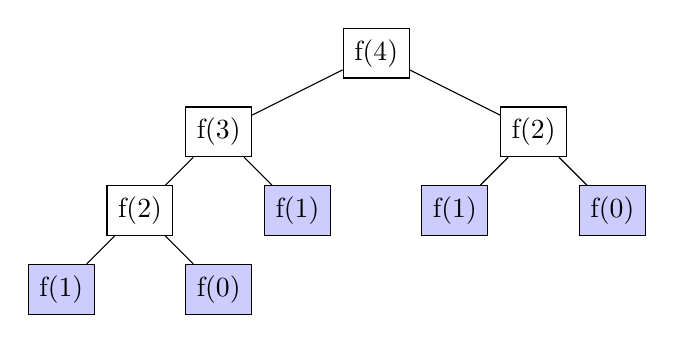
\begin{tikzpicture}[level distance=10mm]
	\tikzstyle{every node}=[fill=white,draw=black,rectangle,inner sep=4pt]
	\tikzstyle{every child}=[fill=white,draw=black,rectangle,inner sep=4pt]
	\tikzstyle{level 1}=[set style ={{every child}+=[sibling distance=40mm]}]
	\tikzstyle{level 2}=[set style ={{every child}+=[sibling distance=20mm]}]
	\node{f(4)}
		child {node {f(3)}
				child{node {f(2)}
					child{node[fill=blue!20]{f(1)}}
					child{node[fill=blue!20]{f(0)}}
				}
				child{node[fill=blue!20] {f(1)}}
			}
		child{node {f(2)}
			child{node[fill=blue!20]{f(1)}} 
			child{node [fill=blue!20]{f(0)}}
			};		
\end{tikzpicture}
\end{center}

An iterative formulation of the above algorithm can also be established and nicely shows the advantage of its recursive brother:

\begin{TPCpp}
// POST: return value is the n-th Fibonacci number F(n)
unsigned int fib2 (const unsigned int n) {
	if (n == 0) return 0;
	if (n <= 2) return 1;
	unsigned int a = 1; // F_1
	unsigned int b = 1; // F_2
	for (unsigned int i = 3; i <= n; ++i) {
		unsigned int a_prev = a; // F_i-2
		a = b; // F_i-1
		b += a_prev; // F_i-1 += F_i-2 -> F_i
	}
	return b;
}
\end{TPCpp}

\section{Arrays}
\label{sec:Arrays}

Arrays are used to save a previously known number of data points of the same type.

\begin{TPCpp}
int list_1 [4]; // [r1 r2 r3 r4]
int list_2 [ ] = {1,2,3,4}; // [1 2 3 4]
int list_3 [4] = {1}; // [1 0 0 0]
list_1 [0] = 1;
//list_1 [4] = 5; // segmentation fault
\end{TPCpp}

\begin{itemize}
\item Arrays are declared with type, name and the length in square brackets. Uninitialized arrays contain random values. (\verb+list_1+)
\item Arrays with undefined length need to be initialized directly such that the length can be determined. (\verb+list_2+)
\item Arrays with a short initialization will fill up with zeros. (\verb+list_3+)
\item Array indexing starts with 0.
\item Accessing out-of-bound values results in undefined behaviour.
\end{itemize}

\subsection{Arrays and Pointers}
\label{sec:ArraysAndPointers}

The name of an array can be understood as a pointer to the first element of the array.

\begin{TPCpp}
int list_1 [4] = {1,2,3,4};
int list_2 [1];
// list_1 = list_2; // error
int * list_pointer_1 = list_1;
int * list_pointer_2 = &list_1[0];
list_1[1]; // value: 2
list_pointer_1[1]; //value: 2
list_pointer_2[1]; //value: 2
*(list_1 + 1); //value: 2
\end{TPCpp}

\begin{itemize}
\item The name of an array is a pointer that is not allowed to be changed.
\item A pointer to the name of an array is equivalent with a pointer to the address of the first element of the same array.
\item The access operator \verb+[]+ works on the array name as well as on a pointer on the array.
\item The access operator is equivalent with the increment and subsequent dereferencing of a pointer to the array.
\end{itemize}

Based on the knowledge that arrays are saved with a pointer to the first element of the allocated memory dynamic arrays can be created:

\begin{TPCpp}
int n;
cin >> n;
int * dynamic_array = new int [n];
\end{TPCpp}

\begin{itemize}
\item The dynamically allocated array can now be used exactly the same as a static array.
\item The dynamic array needs to be deleted with \verb+delete [] dynamic_array+ in order not to create memory leaks!
\end{itemize}

\subsection{Multidimensional Arrays}
\label{sec:MultidimensionalArrays}

Arrays can have more than one dimension, and can thus also be used to represent matrices or tables. 

\begin{TPCpp}
//2 elements, each an array of length 3
//uninitialized
int a_1[2][3];
//initialized, size specified
int a[2][3] = {
	{1,2,3},{2,6,3}
};
//initialized, size partially specified
int a[][3] = {
	{1,3,4},{2,3,4},{13 3 2}
};
\end{TPCpp}

As described in the last example it is possible to leave the first dimension unspecified if a direct initialization follows. Exactly as for simple arrays the length is determined automatically. This however does not work for the second dimension.
The array above is saved in the memory as seen below:

\includegraphics[width=\linewidth]{Pictures/2DArray}

\subsection{Passing Arrays as Arguments}
\label{sec:PassingArraysAsArguments}

Since we know that arrays are basically pointers to memory it is possible to pass an array to the function by simple giving it a pointer to the first element of the array. Using references however we can prevent the decaying of the array-name (which remembers the length of the array if defined statically) by passing a reference to the array name as follows:

\begin{TPCpp}
void some_array_function(int pointer []){
	//...
}

void nice_array_function(int (&arrayname) [10]{
	//...
}
\end{TPCpp}

The first function will accept any pointer and will not preserve the knowledge of the length of the array. The second function is able to determine whether the argument is actually an array of the specified length and will preserve this information, but has the drawback that it only works for that specific length.

\section{vector}
\label{sec:vector}

The vector class is a member of the standard library and improves on many of the issues observed with arrays. Vectors are implemented as a template and thus need a type specification in angled brackets.

\begin{TPCpp}
#include <vector>

std::vector<int> int_vector;
\end{TPCpp}

The basic functionality of vector can be seen here, \easyurl{read}{http://www.cplusplus.com/reference/vector/vector/} for more details.

\begin{TPCpp}
//create a bool vector with length 100
//all entries set to false
std::vector<bool> status(100,false);

//create a copy of an existing vector
std::vector<bool> copy(status);

//access entries
copy[0]; // first entry
copy.at(0); // first entry
copy.push_back(true); // append entry: true
copy.pop_back(); //delete last element
\end{TPCpp}

There also exists the possibility of filling up a vector with a certain value, over a certain interval, defined by two iterators.

\begin{TPCpp}
#include <algorithm>

/*
std::fill(b,p,val) //where b,p are iterators
*/

std::vector<int> vec (5,4);            // vec: 4 4 4 4 4
std::fill(vec.begin()+3, vec.end(),2); // vec: 4 4 4 2 2
\end{TPCpp}

Another member function can find elements with a certain value within a vector and return an iterator to the first instance found. If nothing is found a past-the-end iterator (with respect to the defined interval) is returned.

\begin{TPCpp}
#include <algorithm>

/*
std::find(b,p,val) // where b,p are iterators
*/

using It =std::vector<int>::iterator;
std::vector<int> vec = {8, 1, 0, -7, 7};
// Goal: Find index of -7 in vec: 8 1 0 -7 7
It pos itr = std::find(vec.begin(), vec.end(), -7);
std::cout << (pos itr - vec.begin()) << "\n"; // Output: 3
\end{TPCpp}

Is is even possible to sort vectors from low to high.

\begin{TPCpp}
#include <algorithm>

/*
std::sort(b,e) //where b,e are iterators
*/

std::vector<int> vec = {8, 1, 0, -7, 7};
std::sort(vec.begin(), vec.end()); // vec: -7 0 1 7 8
\end{TPCpp}

And we can find the minimum element of vector easily using:

\begin{TPCpp}
#include <algorithm>

/*
std::min element(b, p) // where b,p are iterators
*/

// Goal: Make sure that all inputs are > 0
std::vector<int> vec;
int i;
while (std::cin >> i)
vec.push back(i);
assert( *std::min element(vec.begin(), vec.end()) > 0 );
// Note: We have to dereference the (r-value-)iterator.
\end{TPCpp}

Note that all the algorithms used above are made for use with the standard template libraries and thus work for other data structures in that library. Also this has only been a small selection of the available functions. See section \ref{sec:StandardTemplateLibrary} for additional information.

\subsection{Multidimensional Vectors}
\label{sec:MultidimensionalVectors}

Multidimensional vectors are similar to multidimensional arrays in functionality. The declaration is a bit more complicated:

\begin{TPCpp}
using namespace std;
vector < vector < int > > a (n, vector<int>(m));
\end{TPCpp}

The above declaration describes a vector of int vectors. The initialization defines the dimensions as follows: The outer vector is of length n and contains vectors of lengths m. Note that the space between \verb>< <> is necessary, since without it the brackets would be interpreted as an operator.

\subsection{Access}
\label{sec:Access}

There exist different methods of accessing the elements of vectors.

\begin{enumerate}
\item \textbf{Random access:} The concept of random access allows accessing any element of a vector with the same effort.

\begin{TPCpp}
//long array (syntax simplified!)
int a [] = {1,2,3,4,5,6,...,100};

//random access:
a[33]; // identical to: *(a+33);
\end{TPCpp}

The random access operation as described above requires a single addition and an implicit multiplication automatically made through pointer arithmetic when adding a number to a pointer.

This access method is really flexible but also costly.
\item \textbf{Sequential access:} This is where sequential access shines, which only requires a simple addition for getting to the next element in an array, but is less flexible since it can only go back an forth in steps of one. Sequential access can be implemented as follows:

\begin{TPCpp}
int a[5] = {1,2,3,4,5};
for (int* p = a; p < a+5; ++P)
	cout<<*p<<" ";
	
//For vectors iterators can be used

\end{TPCpp}
\end{enumerate}

\subsection{Iterators}
\label{sec:Iterators}

Since vectors allocate memory differently than arrays they cannot simply be traversed using a pointer. For that reason and to have an interface for advanced functionality vectors have iterators pointing to their elements.

\begin{TPCpp}
std::vector<int>::const_iterator

std::vector<int>::iterator
\end{TPCpp}

The first version can be used for non-mutating access. It is analogue to a \verb+const int*+ for arrays. The second version allows changing of the elements it points to. 

\begin{TPCpp}
std::vector<int> vec;
vec.push_back(1);
vec.push_back(2);
std::vector<int>::iterator it = vec.begin();

while(it<vec.end()) {
	cout<<*it<<endl;
	it++;
}
\end{TPCpp}

In the above example the member functions \verb+begin()+ and \verb+end()+ are used to initialize and constrain an iterator going through the vector. Access to pointed-to elements and increment of the iterator works just like it does using pointers.

\subsection{Passing Vectors to Functions}
\label{sec:PassingVectorsToFunctions}

By convention of the standard library vectors are passed to functions using two iterators, one to the beginning of a valid part of the vector to be passed and  a second to the ending of the same. This can of course include the whole vector but includes the flexibility of only processing a part of it.

\begin{TPCpp}
std::vector<double> d(100,0);
std::fill(d.begin(),d.end(),1);
\end{TPCpp}

\section{Strings}
\label{sec:Strings}

\subsection{C-style Character String}
\label{sec:CStyleCharacterString}

One possibility to save a string is using an array of chars. By convention character arrays are terminated with \verb+\0+. This serves the purpose of marking the end of a string.

\begin{TPCpp}
//initialisation with string literal
char text = "bool";
//equivalent to:
char text = {'b','o','o','l','\0'};
\end{TPCpp}

\subsection{string}
\label{sec:string}

The modern alternative to char arrays is the \easyurl{string class}{http://www.cplusplus.com/reference/string/string/} in the standard library. It serves the same purpose as the character array but makes handling strings a lot easier. For instance the length of a string does not have to be known at compiletime and can thus also change during runtime.

\begin{TPCpp}
#include <string>
std::string text1 = "bool";
text1.length(); //A string knows its length
//initialize with variable length n
//and fill with 'a'
std:string text2 (n, 'a');
//string understands comparisons
//and many other operations
text1 == text2; 
\end{TPCpp}

\section{Pointers}
\label{sec:Pointers}

Pointers are variables saving addresses of other variables.

\begin{TPCpp}
int a = 6;
//b is a pointer to an int
//and takes the address of a
int * b = &a;

(*b)++; //a == 7
\end{TPCpp}

There are three important operators for pointers:

\begin{itemize}
\item Declaration of a pointer: 

\begin{TPCpp}
//<type> * <name>;
int * pointer;
\end{TPCpp}

\item Adress of a variable:

\begin{TPCpp}
//& <variable>;

int var;
pointer = & var;
\end{TPCpp}

\item Accessing the value pointed to (dereferencing)

\begin{TPCpp}
//want to set var = 7;
//*<initialised_pointer>;
*pointer = 7; //var == 7
\end{TPCpp}
\end{itemize}

\subsection{Pointer Arithmetic}
\label{sec:PointerArithmetic}

In connection with arrays there are more operations possible:

\begin{TPCpp}
int my_array [10];
//Pointer to first element
int my_pointer = my_array;

while(my_pointer<my_array+10){
	//do something
	//increment pointer
	my_pointer++;
}
\end{TPCpp}

As seen in the example above it is possible to do calculations with pointers. This works since the arithmetic operators (\verb.+,-,++,--.) are overloaded to work with pointers. Also relational operators (\verb.<,>,<=,>=,==,!=.) can be directly used.

What happens internally is that the length of the data element pointed to is known by the type of the pointer and thus an increment leads to the desired change in the saved address, such that \verb+my_pointer+ points to one element in the array after the other.

\subsection{Const Pointers}
\label{sec:ConstPointers}

\begin{itemize}
\item A const pointer cannot point to another variable once initialized.
\item A pointer to a const variable cannot change the variable it points to.
\item A nonconst pointer cannot point to a const variable.
\end{itemize}

\textbf{Read from right to left! Read * as  'Pointer to'.}

\vspace{3ex}

\begin{minipage}[t]{0.4\linewidth}
\begin{itemize}
\item \texttt{\textcolor{blue}{int} \textcolor{violet}{*} \textcolor{orange}{iptr} = \&i;}

\textcolor{orange}{iptr:} \textcolor{violet}{Pointer auf} \textcolor{blue}{int}.
\item \texttt{\textcolor{blue}{const int}\textcolor{violet}{ *} \textcolor{orange}{icptr} = \&i;}

\textcolor{orange}{icptr:} \textcolor{violet}{Pointer auf} \textcolor{blue}{const int}.
\item \texttt{\textcolor{blue}{int const} \textcolor{violet}{*} \textcolor{orange}{ic2ptr} = \&i;}

\textcolor{orange}{icptr2}: \textcolor{violet}{Pointer auf} \textcolor{blue}{const int}.
\end{itemize}
\end{minipage}
\hfill
\begin{minipage}[t]{0.5\linewidth}
\begin{itemize}
\item \texttt{\textcolor{blue}{int} \textcolor{violet}{*} \textcolor{red}{const} \textcolor{orange}{iptrc} = \&i;}

\textcolor{orange}{iptrc:} \textcolor{red}{const} \textcolor{violet}{Pointer auf} \textcolor{blue}{int}.
\item \texttt{\textcolor{blue}{const int} \textcolor{violet}{*} \textcolor{red}{const} \textcolor{orange}{icptrc} = \&i;}

\textcolor{orange}{icptrc:} \textcolor{red}{const} \textcolor{violet}{Pointer auf} \textcolor{blue}{const int}.
\end{itemize}
\end{minipage}


\subsection{Additional Information}
\label{sec:AdditionalInformation}

Also see section \ref{sec:ArraysAndPointers} for the connection between pointers and arrays, as well as \ref{sec:CallByReference} to see how pointers can be used to implement call by reference.

Also consider the additional \easyurl{information}{https://www.tutorialspoint.com/cplusplus/cpp_pointers.htm} explaining many advanced uses of pointers.

\subsection{Differences Between Pointers And References}
\label{sec:DifferenceBetweenPointersAndReferences}

\begin{itemize}
\item A pointer can change where it points to.
\item A pointer can be uninitialized, thus point to \verb+NULL+.
\item A pointer has an address itself.
\item There is no such thing as reference arithmetic.
\end{itemize}

\textbf{A reference can be understood as a constant pointer that does not need to be dereferenced.}

\section{References}
\label{sec:References}

A reference is another name for an already existing variable. It has to be initialized when declared and cannot refer to another variable afterwards. \textbf{The object referred to has to exist at least as long as its reference!}

\begin{TPCpp}
int i = 1;
int & ref_to_i = i;
// int & ref_to_nothing; //not allowed!
\end{TPCpp}

In c++ a reference declaration consists of the type which is to referred to, the \verb+operator&+ and the name of the reference, followed by an assignment of a valid L-value. After initialisation \verb+ref_to_i+ can be used exactly the same as \verb+i+!

\vspace{3ex}

Only \verb+const+ references are allowed to refer to R-values!

\begin{TPCpp}
//int & h = 3; // not allowed!
const int & i = 7;
\end{TPCpp}

Only \verb+const+ references can refer to constant variables.

\begin{TPCpp}
const int n = 5;
// int & i = n; // not allowed
const int & i = n; // allowed, read only
\end{TPCpp}

\section{Input/Output}
\label{sec:InputOutput}

C++ I/O occurs in streams, which are sequences of bytes. When bytes flow from a device like a keyboard, a disk drive or a file to main memory this is called an input operation. If bytes flow the other direction, which means from the program to a device like a display screen or a file this is called an output operation.

The most important libraries for basic IO are:

\begin{itemize}
\item \verb+<iostream>+

This file defines \verb+cin, cout, cerr+ and \verb+clog+, which correspond to the standard input, output, unbuffered error and buffered standard error stream.

\item \verb+fstream+

This file declares services for user-controlled file processing.

\item \verb+sstream+
\end{itemize}

\subsection{cout and cin}
\label{sec:CoutAndCin}

\begin{TPCpp}
#include <iostream>

//allows omitting std:: before cout and cin
using namespace std;

int main(){
	//declare variable
	int a;
	//initialise via keyboard input
	cin>>a;
	//print via console
	cout<<a;
}
\end{TPCpp}

These two streams can also be handed to functions which further allows overloading of \verb+<<+ and \verb+>>+, such that for example more elaborate classes can be handed to \verb+cout+ directly. In the example below a suitable overload for a class implementing rational numbers is made:

\begin{TPCpp}
//Stream operator
//PRE: Takes a ostream as an argument
//POST: Prints to the handed ostream
std::ostream& operator<<(std::ostream& os, const Rational & rational)
{
    os << rational.numerator << "/" << rational.denominator;
    return os;
}
\end{TPCpp}

It is important to notice that \textbf{the standard input stream and the standard output stream are unique objects that cannot be copied}! For that reason when handed to an operator as seen above they are handed as references! For an explanation why this operator returns a reference, see section \ref{sec:ChainedOperators}.

\subsection{ifstream and ofstream}
\label{sec:IfstreamAndOfstream}

These two streams allow reading from a file (\verb+ifstream+) and writing to a file (\verb+ofstream+).

In the subsequent subsections we will build up all the code needed for the above described operations. All snippets contribute to the same program and can be run as a whole.

\subsubsection{Opening a File}
\label{sec:OpeningAFile}

First we open a file in the desired mode using the \verb+fstream+ member \verb+open()+ Selectable file modes are:

\begin{itemize}
\item \verb+ios::app+

Append mode. All output to that file to be appended to the end.
\item \verb+ios::ate+

Open a file for output and move the read/write control to the end of the file.
\item \verb+ios::in+

Open a file for reading.
\item \verb+ios::out+

Open a file for writing.
\item \verb+ios::trunc+

If the file already exists, its contents will be truncated before opening the file.
\end{itemize}

\begin{TPCpp}
#include <iostream>
#include <fstream>

using namespace std;

int main(){
	//declare an instance of ifstream
	ifstream infile;
	//open a file
	infile.open("file_name.txt", ios::in);
\end{TPCpp}

\subsubsection{Reading From a File}
\label{sec:ReadingFromAFile}

After having set up the ifstream we can use it just like \verb+cin+ to read information from the file to main memory:

\begin{TPCpp}
	char in;
	string whole_file;
	//extract from file until
	//end of file is reached
	while(!infile.eof()){
		//read next char
		infile>>in;
		//save char in string
		whole_file.push_back(in);
	}
\end{TPCpp}

\subsubsection{Closing a File}
\label{sec:ClosingAFile}

After reading the file we will close it since it is of no further use.

\begin{TPCpp}
	infile.close();
\end{TPCpp}

\subsubsection{Writing to a File}
\label{sec:WritingToAFile}

Now we'd like to write our read and processed file content to another file. First we open a file.

\begin{TPCpp}
	//Declare instance of ofstream
	ofstream outfile;
	//Open a file
	outfile.open("new_textfile.txt",ios::out);
\end{TPCpp}

The we use \verb+outfile+ to write to a new file.

\begin{TPCpp}
	//After opening writing is possible
	while(!whole_file.empty()){
		char temp = whole_file.pop_back();
		//Some kinda caesar code
		temp++;
		//Write to file
		outfile<<temp;
	}	
\end{TPCpp}

After that the file is closed.

\begin{TPCpp}
	outfile.close();
	return 0;
}
\end{TPCpp}

\subsection{sstream}
\label{sec:sstream}

String-Stream is a stream class that can handle strings. Same as the standard in-/out-streams instances of sstream cannot be copied and should be handed by reference. An exemplary use would be emulating cin-input:

\begin{TPCpp}
char c;
std::cin >> c; // e.g. value: 'b'
// stringstream with value "b345e"
std::stringstream s ("b345e"); 
// c gets value 'b' and s is now "345e"
s >> c;
// c gets value '3' (!as char! since type of c is char)
s >> c;
int n;
// n gets value 45 (!as int! since type of n is int)
s >> n;
// (This works since the computer sees that the next
// 2 characters in the string "45e", namely '4' and '5',
// can be used as the int 45. So after this operation
// s is "e".)
\end{TPCpp}

\subsection{Functionality of Streams}
\label{sec:FunctionalityOfStreams}

A stream can have different statuses and there are functions to check the status of a stream:

\begin{TPCpp}
/*
//true if the end of file has been reached
my_stream.eof()
*/

std::stringstream b ("33");
int z;
b >> z; std::cout << b.eof(); 
// true (>> read 33 and reached end of b)
\end{TPCpp}

\begin{TPCpp}
/*
//true if an invalid character has been read
my_stream.fail()
*/

std::stringstream b ("33a");
int z;
// false (>> read 33)
b >> z; std::cout << b.fail(); 
// true (>> ought to read 'a'
b >> z; std::cout << b.fail(); 
// which is not an int.)
\end{TPCpp}

\begin{TPCpp}
/*
//return the next character converted to int
//without extracting it from the stream
my_stream.peek()
*/

std::stringstream num ("3 a");
// Output: 51 and NOT '3'
std::cout << num.peek() << "\n"; 
num >> c;
std::cout << c << "\n"; // Output: '3'
char next = num.peek();
std::cout << next << "\n"; // Output: ' '
num >> c;
std::cout << c << "\n"; // Output: 'a'
\end{TPCpp}

\begin{TPCpp}
/*
std::ws //extract whitespaces until next character
std::noskipws //prevent auto-ignoring of whitespaces
*/

char c;
std::stringstream t ("d a\n\nb");
t >> std::noskipws; // Do not ignore whitespaces.
// Output t without whitespaces
t >> c; std::cout << c; // Output: 'd'
t >> std::ws; // Remove: " "
t >> c; std::cout << c; // Output: 'a'
t >> std::ws; // Remove: "\n\n"
t >> c; std::cout << c; // Output: 'b'
// Output in total: dab
\end{TPCpp}

\section{struct}
\label{sec:struct}

Struct allows the definition of new custom data types.

\begin{TPCpp}
/* 
struct <name> {
	<type> <member_name>;
	.
	.
	.
}<optional_instance_name>;

*/

struct rational{
	int n;
	int d;
}a;

rational b;
\end{TPCpp}

\begin{itemize}
\item Now the new type \verb+rational+ is defined.
\item It can be directly instantiated by inserting one or several (separated with comma) valid identifiers at the end of the struct definition. In this case we made instance \verb+a+.
\item When making new instances afterwards we can use the name of the new type just as we use the basic types.
\item Member variables can be of basic type as well as of custom type, i.e. structures can be nested.
\item Member types can be combined in any way desired.
\end{itemize}

Members can be initialized directly:

\begin{TPCpp}
//uninitialized
rational s;

//member-by-member
rational t = {1,5};

//copy member-by-member
rational u = t; 
\end{TPCpp}

Note that for custom data types not all operators work out of the box. This leads to the idea of overloading operators, as described in section \ref{sec:OperatorOverloading}.

\section{class}
\label{sec:class}

Classes empower the concept of data encapsulation in c++. They are a variant of structs and as such can have member variables as well as member functions. 

\vspace{3ex}

Note that structs basically have the same functionality as classes. They are introduced differently for didactic reasons but actually the single difference between the two is that the members of a struct are public by default and the members of a class a private by default.

\subsection{Object Oriented Programming}
\label{sec:ObjectOrientedProgramming}

The basic idea of object oriented programming is to build software such that it models reality. For that reason the desired functionality is embedded into a set of objects interacting with one another to solve a set task. With object oriented programming come two main advantages:

\begin{itemize}
\item \textbf{Reusability:} Once described the functionality of a class can be instantiated multiple times, inherited from and adapted for the whole inheritance tree in a single place.
\item \textbf{Encapsulation:} Based on the fact that variables can be made private it is possible to hide information from the user or from other parts of the program. This enables a narrow definition of allowed interactions with data, such that invalid access can be prevented by design.
\end{itemize}

\subsection{Basics}
\label{sec:Basics}

\begin{itemize}
\item \textbf{Class:} The definition of an object, introducing a new data type.
\item \textbf{Instance:} Existing copy of the newly defined data type.
\end{itemize}

\subsection{Class Members}
\label{sec:ClassMembers}

There are two types of class members: \textbf{member functions} and \textbf{member variables}. Member variables are data points within the class. Member functions can access these data points for processing. The members of a class exist in instances of the class.

\begin{TPCpp}
/*
class <class_name> {
	//member variable
	<type> <member_name>;
	//member function
	<rtype> <member_fun_name> ();
	
}<optional_instance_name>;
*/
class Vector {
	//member defintion
}a;
\end{TPCpp}

As seen above instances of a class can be directly added to the class definition.

\begin{TPCpp}
int main(){
	Vector b;
}
\end{TPCpp}

Alternatively the class name can be used as a type specifier, for introducing a new instance.

\subsubsection{Member Functions}
\label{sec:MemberFunctions}

The declaration of a member function always has to take place within the class definition. However it is possible to separate declaration and definition and thus the definition can be placed outside the class definition.

\begin{TPCpp}
class Vector {
public:
	void print();
	void explode(){
		cout<<"BOOM!"<<endl;
	}
};

Vector::print(){
	cout<<"Don't mind me, I'm just printing."<<endl;
}
\end{TPCpp}

The external definition needs to know that is is a member function of the class. This is done using \verb1Vector::1.

\vspace{3ex}

Note that member functions can be declared const, which means that they cannot change any of the members unless they are mutable (see section \ref{sec:StorageClasses}).

\begin{TPCpp}
class Vector {
public:
	void doNothing() const { //nothing }
};
\end{TPCpp}

The const after the parameter list of the function is refering to the implicit \verb+*this+ argument (see section \ref{sec:ThisPointer})  which is accessed by every member function of class.

\subsection{Class Access Modifiers}
\label{sec:ClassAccessModifiers}

Class members, not yet considering inheritance, can be either private or public.

\begin{itemize}
\item Public members are accessible from outside.
\item Private members are only accessible through member functions.
\end{itemize}

\textbf{If there is no access modifier all members of a class are private by default!}

\begin{TPCpp}
class Vector {
	//default: private
	double x; //is private
private: 
	double y; //is private
public:
	void print(); //is public
};
\end{TPCpp}

\subsubsection{Access Methods}
\label{sec:AccessMethods}

In order to define an interface to the hidden data one often defines get- and set-functions:

\begin{TPCpp}
	//within definition of vector
	double get_x() const {return x;}
	double get_y() const {return y;}
	
	void set_x(const double _x) {x = _x;}
	void set_y(const double _y) {y = _y;}
\end{TPCpp}

\subsubsection{Access Operators}
\label{sec:AccessOperators}

When accessing the members of a class not from within the class but from the outside, through an instance, there exist two operators managing access to public members:

\begin{TPCpp}
//Instance of Vector
Vector a;
//Pointer of type Vector to a
Vector * pointer = &a;

//Direct access operator .
a.set_x(7);

//Indirect access operator ->
pointer->set_x(7);
\end{TPCpp}

The \verb+operator.+ is used in connection with an instance of a class. It directly accesses the appended member. The \verb+operator->+ is used for accessing the members of an instance through a pointer. In addition to member access it dereferences the pointer.

\subsubsection{This Pointer}
\label{sec:ThisPointer}

Sometimes it is useful to have access to the instance of a class as an object, not only to its members. In that case the \verb+this+ pointer comes in handy. It is a pointer saving the address of the instance it is used in. Thus the above defined access methods could also look like this:

\begin{TPCpp}
void get_x() const {return this->x;}
void get_y() const {return (*this).y;}
\end{TPCpp}

\subsection{Constructors}
\label{sec:Constructors}

\begin{itemize}
\item Standard member function, exists in default form if not overwritten.
\item Used to initialize member variables.
\item Automatically called upon instantiation.
\item Carries the name of the class.
\item Can be overloaded for different types of initializations.
\item The default constructor does not initialize anything.
\end{itemize}

\begin{TPCpp}
class Vector {
	double x,y;
public:
	//Overwriting the default constructor
	Vector (){
		x = 0;
		y = 0;
	}
	//Overloading the constructor
	Vector (double _x, double_y)
		: x(_x),y(_y) {}
}
\end{TPCpp}

The above implementation of the constructor overload makes use of the so called \textbf{initializer list} which is a list of member variables and their respective value in brackets. This comes in especially handy if a class has const members that cannot be initialized within the function body.

\subsubsection{Copy Constructor}
\label{sec:CopyConstructor}

The copy constructor is used for:

\begin{itemize}
\item Initializing one object from another of the same type.
\item Copying an object to pass it as an argument to a function.
\item Copying an object to return it from a function.
\end{itemize}

The default copy constructor simply sets the member variables of the target equal with those of the source. This is not sufficient if a class has dynamic memory allocated.

\begin{TPCpp}
/*
<classname> (const <classname> & obj) {
	//body of constructor
}
*/

Vector (const Vector& obj){
	this->x = obj.x;
	this->y = obj.y;
}
\end{TPCpp}

\subsection{Destructor}
\label{sec:Destructor}

\begin{itemize}
\item Standard member function, exists in default form if not overwritten.
\item Used to deallocate memory taken by an instance.
\item Is called whenever an instance is explicitly deleted or reaches end of scope.
\item The destructor only needs to be overwritten in case the class allocates dynamic memory.
\end{itemize}

\begin{TPCpp}
/*
~<classname> (){
	delete <dynamic_variable>;
	delete [] <dynamic_array>;
}
*/

~Vector (){
	cout<<"Vector is being destructed."<<endl;
}
\end{TPCpp}

For the lack of dynamically allocated memory the default constructor of Vector has been overloaded with this simple output, an easy way to see when the destructor is called.

\subsection{friend}
\label{sec:friend}

To allow a non-member function full access to the private variables of a class, friend functions can be defined as follows:

\begin{TPCpp}
//outside class
void foreign_print(Vector obj){
	cout<<obj.x<<" "<<obj.y;
}

//inside class

friend void foreign_print(Vector obj);
\end{TPCpp}

\subsection{Static Members}
\label{sec:StaticMembers}

A static member of a class exists only once, independent of how many instances of that class are around. All instances work with one and the same static variable.

\begin{TPCpp}
static <member_type> <member_name>;
\end{TPCpp}

\section{Dynamic Data Structures}
\label{sec:DynamicDataStructures}


To illustrate the consequences of dynamic memory allocation in a custom data type, the example of a stack is shortly covered.

\subsection{Linked List}
\label{sec:LinkedList}

The idea of a linked list is to enhance the capability of a simple array with more flexibility. We want to have the freedom to:

\begin{itemize}
\item Insert/Append data points
\item Remove data points
\end{itemize}

This is achieved using so called linked lists, which in their simplest form are based on the following struct, in this case built for integer data points.

\begin{TPCpp}
struct node {
	int datum;
	node * next;
}
\end{TPCpp}

Now the idea of a linked list:

\begin{enumerate}
\item Start the list with your first data point. Let its member \verb+next+ point to \verb+NULL+. This is the end of our list.
\item Append a new data point by allocating it dynamically and setting its \verb+next+ pointer to the address of the old starting point of our list.
\item Always save a pointer to the start of the list. This is all the information needed to access all points in the list.
\item Traverse through the list by subsequently accessing the \verb+next+ pointers.
\end{enumerate}

This is the idea of a singly linked list (linked in one direction) that can be used to implement a stack. The concept however allows \easyurl{much more}{https://www.geeksforgeeks.org/data-structures/linked-list/}.

\subsection{Stack}
\label{sec:Stack}

The stack is a so called FIFO (First in first out) data structure. It can be associated with a stack of bricks. The one laid on top has to be removed again first.

\begin{TPCpp}
class stack {
public:
	void push (int value);
	int pop ();
	void print();
private:
	node* top_node;
}
\end{TPCpp}

Our stack can now be used as follows:

\begin{TPCpp}
stack s1;
s1.push(1);
s1.push(3);
s1.push(2);
\end{TPCpp}

\subsection{Copy Constructor}
\label{sec:CopyContstructorDynamic}

Now if we use the standard copy constructor for our stack, our only member variable is copied, such that now we have two stacks using the same set of nodes:

\begin{TPCpp}
stack s2(s1);
\end{TPCpp}

\includegraphics[width=\linewidth]{Pictures/Stack1}

The issue is that if now \verb+s1+ pops one of the nodes \verb+s2+ will be pointing to a now inexistent node. In other words the two stacks are not independent. To resolve this the copy constructor is overwritten as follows:

\begin{TPCpp}
stack::stack(const stack& s) : top_node (0) {
	copy(s.top_node, top_node);
}

void stack::copy(const node* from, node*& to) {
	assert (to == 0);
	if (from != 0) {
		to = new node(from->datum);
		copy(from->next, to->next);
	}
}
\end{TPCpp}

\subsection{Assignment operator}
\label{sec:AssignmentOperatorDynamic}

Now assume we'd like to assign one stack to another:

\begin{TPCpp}
stack s2;
s2.push(4);
s2.push(9);
s2 = s1;
\end{TPCpp}

\includegraphics[width=\linewidth]{Stack2}

The problems arising here are:

\begin{itemize}
\item We have two non-independent stacks againg.
\item The nodes 9 and 4 of former \verb+s2+ are memory leaks.
\end{itemize}

To solve this the assignment operator is overloaded. First we need a function cleaning up memory leaks:

\begin{TPCpp}
void stack::clear(node* from) {
	if (from != 0) {
		clear (from->next);
		delete from;
	}
}
\end{TPCpp}

\begin{TPCpp}
stack& stack::operator= (const stack& s) {
	if (top_node != s.top_node) { // test for self-assignment
		clear(top_node);
		top_node = 0; // fix dangling pointer
		copy(s.top_node, top_node);
	}
	return *this;
}

\end{TPCpp}

\subsection{Destructor}
\label{sec:DestructorDynamic}

The final issue that needs to be addressed is the case when a stack is at the end of its scope and thus deleted. The standard destructor will just delete all member variables, and thus not clean up our dynamically allocated nodes. To solve this the destructor is overwritten as well:

\begin{TPCpp}
stack::~stack() {
	clear(top_node);
}
\end{TPCpp}

\subsection{Rule of three}
\label{sec:RuleOfThree}

\textbf{If a class defines one or more of the following it should probably define all of them:}

\begin{itemize}
\item destructor
\item copy constructor
\item copy assignment operator
\end{itemize}

All three functions above are compiler generated, thus exist automatically in their naïve default version. If one of them has been overwritten it means that the compiler made version does not suit the need of the underlying class. Thus it is very likely that the other two are not suitable as well.

\section{Inheritance}
\label{sec:Inheritance}

The concept of inheritance allows building a class upon another, such that the basis inherits all its members to a derived class. This allows reusing code and reduces the amount of code written if multiple similar objects are needed. Further, if the basic traits of a family of objects need to be changed, if implemented correctly only the base class needs to be adapted.

\begin{TPCpp}
class A{	//base class
	//... 
};

//derived class
class B : public A {
	//...
};
\end{TPCpp}

\subsection{Access Control and Inheritance}
\label{sec:AccessControlAndInheritance}

As classes have members with different access specifications there needs to be a way to define which member is available in what way in a derived class. This is done with the table below. The access specifier of the inherited member is on the horizontal direction. The type of inheritance is on the vertical direction.

\begin{center}
\begin{tabular}{|l|lll|}
\hline
Inheritance \verb+\+ Member & \verb+public+ & \verb+protected+ & \verb+private+\\\hline
\verb+public+&\verb+public+&\verb+protected+&n/a\\
\verb+protected+&\verb+protected+&\verb+protected+&n/a\\
\verb+private+&\verb+private+&\verb+private+&n/a\\\hline
\end{tabular}
\end{center}

The type of inheritance is incorporated in the definition of the derived class as follows:

\begin{TPCpp}
class base {
private:
	int pr_member;
public:
	int pu_member;
};

/*
class <derived_name> : <access modifier> <base_name> {
	//...
};
*/

class derived : private base {
	// pr_member not available
	// pu_member available as private
};
\end{TPCpp}

\subsection{Constructors}
\label{sec:ConstructorsInheritance}

Since private member variables are not accessible in derived classes, they need to be initialized differently:

\begin{TPCpp}
class base{
	int Bvar;
public:
	base(int _Bvar) : Bvar(_Bvar){}
};

class deri = public base {
	int Dvar;
public:
	deri(int _Bvar, int _Dvar) : base(_Bvar), Dvar(_Dvar) {}
};
\end{TPCpp}

\subsection{is a - has a}
\label{sec:IsAHasA}

Classes can inherit from each other or they can contain each other as member variables.

\begin{TPCpp}
class University {
private:
	std::vector<Student> students_;
};

class Student {
private:
	Legi legi_;
};

class Phys_Student : public Student {};

class Legi {
	int immatriculation_year_;
};
\end{TPCpp}

The above set of classes show the difference. A university \textbf{has} students. A physics student \textbf{is} a student. In implementation both versions can be used and yield very similar results. The decision which to choose is often based on the reality that is to be represented.

\subsection{Polymorphism}
\label{sec:Polymorphism}

Polymorphism is a concept based on the possibility to let pointers of the type of the base class point to derived classes.

\begin{TPCpp}
class base {
	//...
};

class derived : public base {
	//...
};

derived derived_instance;
base * pointer = &derived_instance;
\end{TPCpp}

When now this pointer is used to call a member function defined in the base class and overwritten in the derived class, the decision which version to use needs to be made. Normally the member function, that is associated with the type of the pointer (thus base class) will be executed.

\subsubsection{virtual}
\label{sec:virtual}

This behaviour can be changed when a function is declared as virtual in the base class. Then a pointer of the base class, pointing to a derived class, will use the function definition within the derived class. This is called \textbf{dynamic binding}.

\begin{TPCpp}
class A {
	virtual void print() 
	{cout<<"A"<<endl;}
};

class B : public A {
	void print()
	{cout<<"B"<<endl;}
};

A instantce1;
instance1.print(); // "A"
B instance2;
instance2.print(); // "B"
A * pointer1 = &instance2;
pointer1->print(); // "B"
\end{TPCpp}

This behaviour can be summed up as follows:

\begin{enumerate}
\item When called directly, via an instance of a class, the member function corresponding to the type of the calling instance is used.
\item When a non-virtual member function is called indirectly, via a pointer to an instance, the function corresponding to the type of the calling pointer is used.
\item When a virtual member function is called indirectly, via a pointer an instance, the function corresponding to the type of the calling instance is used.
\end{enumerate}

\ifnum\conditionmacro=1
\subsubsection{\ntn{Abstract Base Class}}
\label{sec:AbstractBaseClass}

Normally functions need to be defined at some point. For virtual functions however it is possible to omit the definition entirely, setting them to zero.

\begin{TPCpp}
class base  {
	virtual void print() = 0;
}
\end{TPCpp}

Now since this function is undefined to this point, the base class holding it can not be instantiated. Further this class is now called \textbf{abstract base class} since it holds a \textbf{pure virtual function}.

\begin{TPCpp}
class derived : public base {
	void print() {
		cout<<"derived"<<endl;
	}
};

//base instance1; //forbidden
base * pointer1 = new derived; //allowed
\end{TPCpp}
\fi

\section{Overloading}
\label{sec:Overloading}

Functions and operators can work differently, depending on their arguments or operands.

\subsection{Function Overloading}
\label{sec:FunctionOverloading}

Functions overloading means varying the types, the order and the number of arguments given to the function. For each variation a different behaviour can be programmed. Upon call the handed arguments are compared with the overload signatures and the matching function is executed. If no matching function is found \easyurl{overload resolution rules}{https://en.cppreference.com/w/cpp/language/overload_resolution} are applied.

\begin{TPCpp}
//a way of identifying unknown variable types:

void identify (int a){
	cout<<"My type is int."<<endl;
}

void identify (double a){
	cout<<"My type is double."<<endl;
}
\end{TPCpp}

Based on the rule stated above the following overloads are possible:

\begin{TPCpp}
void fun();			//without argument
void fun(int a);	//with argument
void fun(double b); //different type
//different number of arguments
void fun(int a, int b);
//different type of arguments
void fun(int a, double b);
//different order of arguments
void fun(double b, int a);
\end{TPCpp}

Based on the above the following overloads are not valid:

\begin{TPCpp}
//No distinction by return type
int fun();
//No distinction by argument name
int fun(int different);
\end{TPCpp}

\subsection{Operator overloading}
\label{sec:OperatorOverloading}

Operators are can be described like functions. Depending on their definition they have a set of arguments, i.e. left-hand side and right-hand side for \verb-operator+- and a return value connected to a post condition, which in this case would be: returns the sum of the two handed variables. As done above, in c++ operators can be addressed via their name and the keyword \verb+operator+ in front.

\vspace{3ex}

Based on that idea it is obvious that overloads are also possible for operators, which allows defining them also for our custom data types. Thus an operator overload is defined as a normal function, using \verb+operator<name>+ as a function name, and defining the argument list such that it fits the chosen operator.

\vspace{3ex}

There is a binary \verb+operator-+ and a unary \verb+operator-+. To show how they differ in their signature the following example is established for the custom data type \verb+rational+.

\begin{TPCpp}
struct rational{
	int n;
	int d;
};
\end{TPCpp}

The overloading of the binary operator, taking the value on its left and the value on its right:

\begin{TPCpp}
rational operator- (const rational& l, const rational& r){
	rational result;
	result.n = l.n*b.r - l.d*r.n;
	result.d = l.d*b.r;
	return result;
}
\end{TPCpp}

The overloading of the unary \verb1operator-1, taking the value on its right. 

\begin{TPCpp}
rational operator- (const rational& r){
    rational result = r;
	result.n = -result.n;
	return result;
}
\end{TPCpp}

Note that the parameters are handed as const references, therefore they are not changed by accident and rather than copying the whole structure a referenced is handed to the function.

Both operators in use:

\begin{TPCpp}
int main(){
	rational a = {1,3};
	rational b = {2,4};
	//unary operator-
	rational c = -b; // -2/4
	//binary operator-
	rational d = a-b;
}
\end{TPCpp}

\subsubsection{Overloadable Operators}
\label{sec:OverloadableOperators}

\begin{TTable}{*{6}{p{0.1\linewidth}}}
\verb-+-&\verb+-+&\verb+*+&\verb+/+&\verb+%+&\verb+^+\\
\verb+&+&\verb+|+&\verb+~+&\verb+!+&\verb+,+&\verb+=+\\
\verb+<+&\verb+>+&\verb+<=+&\verb+>=+&\verb-++-&\verb+--+\\
\verb+<<+&\verb+>>+&\verb+==+&\verb+!=+&\verb+&&+&\verb+||+\\
\verb-+=-&\verb+-=+&\verb+/=+&\verb+%=+&\verb+^=+&\verb+&=+\\
\verb+|=+&\verb+*=+&\verb+<<=+&\verb+>>=+&\verb+[]+&\verb+()+\\
\verb+->+&\verb+->*+&\verb+new+&\verb+new[]+&\verb+delete+&\verb+delete[]+\\
\end{TTable}

Note that there are certain operators that cannot be overloaded:

\begin{TTable}{*{4}{p{0.1\linewidth}}}
\verb+::+&\verb+.*+&\verb+.+&\verb+?:+\\
\end{TTable}

Find examples for the overloading of any of the operator types listed above \easyurl{here}{https://www.tutorialspoint.com/cplusplus/cpp_overloading.htm}

\subsubsection{Chained operators}
\label{sec:ChainedOperators}

Certain operators allow to be chained together. Good examples are the assignment operator or the I/O operators \verb+<<+ and \verb+>>+. To preserve the ability to be put in chains, these operators need to return references. Why this is necessary will become obvious in the following example:

\begin{TPCpp}
#include <iostream>

using namespace std;

cout<<"Hello"<<" world"<<'!'<<endl;
\end{TPCpp}

The \verb+operator<<+ is left-to-right associative, therefore its first evaluated occurrence is \verb+cout<<"Hello"+. This term has to return a reference to the standard output stream such that the next evaluation \verb+cout<<" world"+ can be made properly.

\begin{TPCpp}
std::ostream& operator<< (std:ostream& out, rational r){
	return out << r.n << "/" << r.d;
}
\end{TPCpp}

\section{Dynamic Memory}
\label{sec:DynamicMemory}

Normally memory is allocated according to the variables specified, before program execution. However it is often practical to allocate memory during runtime.

\begin{itemize}
\item Every \verb+new+ needs a fitting \verb+delete+.
\item Not cleaning up leads to memory leaks which can finally fill up the heap (heap overflow).
\end{itemize}

\subsection{new}
\label{sec:new}

\begin{TPCpp}
/*	
	new <type> (<constructor args>);
*/

//allocation of a single variable
int * pointer;
pointer = new int;

//allocation of a whole array
//length does not have to be defined
//at compiletime!
int * another_pointer;
another pointer = new int [length];
\end{TPCpp}

\begin{itemize}
\item \verb+new+ allocates a new object of the desired type, calls the correct constructor as specified in the brackets and returns a pointer to the newly generated object. If no constructor is needed the brackets can be omitted.
\end{itemize}

\subsection{delete}
\label{sec:delete}

Object that are allocated using \verb+new+ have dynamic storage duration, the memory occupied by them is only released again if explicitly deleted.

\begin{TPCpp}
/*
	delete <pointer>
*/

//delete the objects allocated above
delete pointer;

//Use delete [] for dynamically allocated arrays
delete [] another_pointer;
\end{TPCpp}

\begin{itemize}
\item \verb+delete+ removes dynamically allocated objects.
\item \verb+delete+ needs a pointer to the object in order to delete it.
\end{itemize}

\section{Namespaces}
\label{sec:Namespaces}

\begin{itemize}
\item Different libraries using the same function name call for a distinction.
\item \verb+namespace+ allows wrapping declarations in an envelope that distinguishes them from any definition with the same name.
\item With \verb+using namespace <namespace_name>+ the compiler is informed that functions from that namespace are used. This does not work if we introduce ambiguities:
\item If we were \verb+using namespace n1;+ in the example below, there would be an ambiguous function overload, which leads to a compilation error.
\item Namespaces can be discontiguous, i.e. split into different parts in different files. If part of the namespace requires a name defined in another file, that name must still be declared!
\item There can be namespaces inside namespaces.
\end{itemize}

\begin{TPCpp}
/*	
namespace <namespace_name> {
	// code declarations
}
*/

namespace n1 {
	void myfun(){cout<<"n1";}
}

void myfun(){cout<<"outside";}

//using namespace n1; //error

int main(){
	myfun(); //outputs "outside"
	n1::myfun(); //outputs "n1"
}
\end{TPCpp}

\ifnum\conditionmacro=1
\section{\ntn{Templates}}
\label{sec:Templates}

Templates are the foundation of generic programming, which in different terms is the practice of writing code in a way that is independent of any particular data type. A template can be understood as a blueprint or a formula for creating a generic class or function. The first example of templates we got to enjoy was \verb+vector+ which was always handed its specific data type via angled brackets.

\subsection{\ntn{Template Function}}
\label{sec:TemplateFunction}

\begin{TPCpp}
/* general form of a template
template <class type> ret-type func-name(parameter list) {
	// body of function
}
*/
template <typename T>
T const& Max(T const& a, T const& b){
	return a<b ? b:a;
}
\end{TPCpp}

In the example above we defined a function template \verb+Max+ that can now be used for any data type that has suitable overloading for the used operators. Without templates we would need to overload \verb+Max+ for every new datatype we'd like to feed it. When called a template function can recognize the data type it is fed and in contrast to template classes it does not need to be told explicitly what data type to expect as you can see below:

\begin{TPCpp}
int main(){
	int j = 29;
	int k = 20;
	Max(i,j); //returns 29
	
	string s1 = "Hello";
	string s2 = "World";
	Max(s1,s2); //return "World";
\end{TPCpp}

\subsection{\ntn{Template Class}}
\label{sec:TemplateClass}

\begin{TPCpp}
/* general form a of a template class
template <class type> class class-name{
	//class contents
}
*/

//in the header file
template <class T>
class Stack {
private:
	vector<T> elements;
public:
	//push element
	void push(T const&);
	//pop element
	void pop();
	//return top element
	T top() const;
	//return true if empty
	bool empty() const;
}
\end{TPCpp}

Above we have declared a template class that can handle stacks of any variable type we choose. Now we need to see how member functions are defined in this case:

\begin{TPCpp}
//in the cpp file
template <class T>
void Stack<T>::push (T const& element){
	// append copy of passed element
	elements.push_back(element);
}
\end{TPCpp}

After having defined all member functions we can use our stack as follows:

\begin{TPCpp}
Stack<int> intStack;

//manipulate our intStack
intStack.push(7);
cout << intStack.top() << endl;

Stack<string> stringStack;

stringStack.push("hello");
stringStack.push("world");
cout<<stringStack.top();
stringStack.pop();
cout<<stringStack.top();
//we just made ourselves 
//a nice implementation of hello world ;)
\end{TPCpp}
\fi

\section{Standard Template Library}
\label{sec:StandardTemplateLibrary}

The C++ STL (\easyurl{Standard Template Library}{https://www.tutorialspoint.com/cplusplus/cpp_stl_tutorial.htm}) is a powerful set of C++ template classes to provide general-purpose classes and functions with templates that implement many popular and commonly used algorithms and data structures like vectors, lists, queues, and stacks.

\end{multicols*}
\end{document}
